\chapter{Fundamentação Teórica}

Este capítulo apresenta os fundamentos teóricos que embasam este trabalho, abrangendo tanto os aspectos físicos associados ao processo de destilação por membranas quanto os conceitos de aprendizado de máquinas utilizados na modelagem baseada em dados. Inicialmente, são discutidos os princípios de funcionamento da destilação por membranas e os mecanismos de transporte de massa e calor que governam o processo, bem como a formulação de modelos físicos reduzidos. Em seguida, são apresentados os principais conceitos de aprendizado supervisionado, incluindo formulação de problemas de regressão, métricas de avaliação, estratégias de validação e controle de complexidade. Por fim, são descritas as principais famílias de modelos utilizadas, assim como abordagens híbridas que integram conhecimento físico e aprendizado de máquina, estabelecendo a base conceitual para a metodologia adotada neste trabalho.



\section{Destilação por Membranas}

\subsection{Princípios Físicos}

Conforme discutido anteriormente, a destilação por membranas é baseada na migração de vapor de água através de uma membrana hidrofóbica, impulsionada por uma diferença de pressão parcial de vapor entre a solução salina aquecida e uma região fria. Nesta seção, retomam-se apenas os princípios físicos relevantes para a compreensão do processo e das variáveis utilizadas na modelagem desenvolvida neste trabalho. A força motriz do processo decorre do gradiente térmico estabelecido entre a alimentação aquecida e uma região de menor temperatura, o que gera uma diferença de pressão de vapor ao longo da membrana. A membrana atua como uma barreira não molhável ao escoamento do líquido, permitindo apenas a passagem do vapor d'água. O mecanismo fundamental envolve evaporação na interface do lado quente, transporte do vapor através dos poros da membrana e posterior remoção ou condensação do vapor, dependendo da configuração de MD considerada (\cite{Cath2010, Hitsov2015}).

A força motriz do processo decorre do gradiente térmico estabelecido entre a corrente quente de alimentação e a corrente fria de condensação, o que gera uma diferença de pressão de vapor ao longo da membrana. A membrana atua como uma barreira não molhável ao escoamento do líquido, permitindo apenas a passagem da fase vapor. O mecanismo fundamental envolve evaporação na interface do lado quente, difusão do vapor através dos poros da membrana e posterior condensação no lado frio (\cite{Cath2010, Hitsov2015}).

Diversas configurações de MD são descritas na literatura, diferenciando-se principalmente pela forma como o vapor é removido e condensado após atravessar a membrana (\cite{Cath2010, Warsinger2017, AlZoubi2018, Chong2022}). As quatro configurações básicas mais recorrentes são:

\begin{itemize}
    \item \textit{Direct Contact Membrane Distillation} (DCMD): as correntes quente e fria entram em contato direto com os lados opostos da membrana. Apresenta construção simples e condensação interna do vapor, mas pode sofrer maiores perdas térmicas por condução através da membrana.

    \item \textit{Air Gap Membrane Distillation} (AGMD): há um espaço de ar de ar entre a membrana e a superfície de condensação. Essa configuração reduz perdas térmicas por condução e permite a condensação interna do permeado, mas o espaço de ar adiciona resistência ao transporte de massa, podendo reduzir o fluxo de permeado.

    \item \textit{Vacuum Membrane Distillation} (VMD): aplica-se vácuo no lado do permeado, removendo o ar e reduzindo a resistência difusiva ao transporte de vapor. Embora possa favorecer maiores fluxos de permeado, essa configuração exige condensação externa do vapor produzido, aumentando a complexidade do sistema.

    \item \textit{Sweeping Gas Membrane Distillation} (SGMD): utiliza-se um gás de arraste no lado do permeado para remover o vapor que atravessa a membrana. Essa configuração reduz a pressão parcial de vapor no lado do permeado, mas também requer condensação externa e controle adicional do escoamento do gás.
\end{itemize}

Além dessas configurações básicas, existem arranjos derivados que combinam características de mais de uma configuração. Entre eles, destaca-se a \textit{Vacuum-Enhanced Air Gap Membrane Distillation} (V-AGMD), adotada neste trabalho, que combina o espaço de ar de ar característico da AGMD com operação sob pressão reduzida. Essa configuração busca reduzir a resistência ao transporte de massa, mantendo a condensação interna no módulo, o que pode favorecer o desempenho do sistema sem exigir condensação externa do permeado (\cite{Lisboa2024}).

% CITAÇÃO NECESSÁRIA: Verificar se Lisboa2024 ou outra referência específica sustenta diretamente a descrição da configuração V-AGMD e suas vantagens operacionais.
% FIGURA OPCIONAL: Inserir figura esquemática comparando DCMD, AGMD, VMD e SGMD, caso haja uma fonte adequada ou figura autoral.

A escolha da configuração influencia diretamente os mecanismos dominantes de transferência de massa e calor e, consequentemente, o desempenho térmico e energético do sistema \cite{Warsinger2017,Hitsov2015}.
\subsection{Modelagem do Transporte de Massa}

Como este trabalho trata de um sistema V-AGMD, a descrição do transporte de massa é direcionada às configurações AGMD e V-AGMD. Nessas configurações, o vapor formado na interface entre a solução salina aquecida e a membrana atravessa os poros da membrana e, em seguida, percorre uma região gasosa até a superfície de condensação. No caso da V-AGMD, esse transporte ocorre sob pressão reduzida, o que altera a resistência difusiva associada à presença de ar no domínio gasoso.

O transporte de vapor através da membrana pode ser descrito pelo modelo de \textit{Dusty Gas}, uma formulação que contempla diferentes contribuições ao transporte em meios porosos, incluindo difusão molecular, difusão de Knudsen, difusão superficial e escoamento viscoso ou convectivo nos poros. No entanto, a depender das condições do sistema e das hipóteses simplificadoras adotadas, algumas dessas contribuições podem ser desconsideradas. No modelo utilizado como referência neste trabalho, considera-se a combinação entre difusão molecular e difusão de Knudsen, enquanto efeitos associados à difusão superficial e ao escoamento viscoso do tipo Poiseuille são negligenciados (\cite{Lisboa2024}).

\begin{figure}[H]
    \centering
    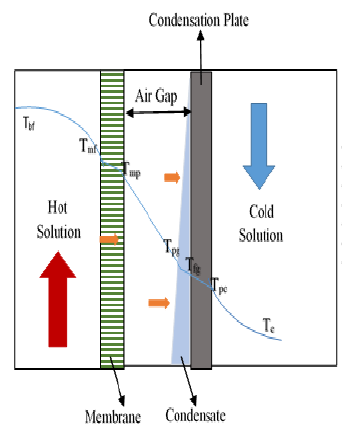
\includegraphics[width=0.5\linewidth]{Imagens/chap03/Model-of-heat-and-mass-transfer-in-the-AGMD.png}
    \caption[Domínio considerado na modelagem do transporte de massa em AGMD/V-AGMD]{Representação esquemática do domínio considerado na modelagem do transporte de massa em configurações AGMD e V-AGMD, incluindo a interface de evaporação, os poros da membrana, o espaço de ar gasoso e a superfície de condensação.}
    \fonte{Autor: \cite{Zheng2017}}
    \label{fig:dominio_transporte_agmd_vagmd}
\end{figure}

A formulação geral pode ser escrita como

\begin{equation}
\frac{N_w}{D_w^k} + \frac{p_a N_w - p_w N_a}{D_{wa}^0}
=
-\frac{1}{R T_m}\frac{d p_w}{dx}
\end{equation}

\noindent em que \(N_w\) é o fluxo molar de vapor de água, \(D_w^{K}\) é a difusividade de Knudsen, \(D_w^{M}\) é a difusividade molecular do vapor de água no ar, \(p_w\) e \(P\) são, respectivamente, a pressão parcial do vapor de água e a pressão total do sistema, \(R\) é a constante universal dos gases e \(T_m\) é a temperatura média na membrana.

Assumindo ausência de fluxo molar de ar \((N_a \approx 0)\), a expressão pode ser simplificada e, após integração ao longo da espessura da membrana \(\delta_m\), obtém-se uma forma funcional para o fluxo mássico de permeado \(j_w\):

\begin{equation}
j_w = \frac{M_w D_{wa}^{0}}{R T_m \delta_m}
\ln \left(
\frac{D_{wa}^{0} - D_{\mathrm{eff}} p_{mg}}
{D_{wa}^{0} - D_{\mathrm{eff}} p_{mf}}
\right)
\end{equation}

\noindent em que \(M_w\) é a massa molar da água, \(p_{mf}\) é a pressão parcial de vapor na interface entre a solução salina aquecida e a membrana, e \(p_{mg}\) é a pressão parcial de vapor junto à superfície fria de condensação, localizada após o espaço de ar gasoso. Nas configurações AGMD e V-AGMD, essa superfície corresponde à região onde se forma o filme de água condensada. Dessa forma, a diferença de temperatura entre a interface da solução salina aquecida e a superfície de condensação estabelece o gradiente de pressão parcial responsável pela evaporação e pelo transporte de vapor através da membrana e do espaço de ar.

Para pequenas diferenças de pressão parcial, a expressão pode ser linearizada como

\begin{equation}
j_w = B_m (p_{mf} - p_{mg})
\end{equation}

em que $B_m$ representa o coeficiente global de transferência de massa da membrana.

No espaço de ar, o transporte difusivo pode ser descrito por

\begin{equation}
j_w = B_g (p_{mg} - p_{gl})
\end{equation}

onde $B_g$ é o coeficiente de transferência de massa no air gap e $p_{gl}$ é a pressão parcial de vapor na interface do condensador. Considerando resistências difusivas em série:

\begin{equation}
\frac{1}{B_{eq}} = \frac{1}{B_m} + \frac{1}{B_g}
\end{equation}

resultando em

\begin{equation}
j_w = B_{eq} (p_{mf} - p_{gl})
\end{equation}

A presença de sal na alimentação reduz a pressão de vapor da água. Esse efeito é frequentemente incorporado por meio da atividade da água $a_w$, de forma que

\begin{equation}
p_{mf} = a_w (1 - x_{salt}) p_v
\end{equation}

onde $x_{salt}$ é a fração molar de sal e $p_v$ é a pressão de saturação do vapor, geralmente obtida pela equação de Antoine.

\subsection{Modelagem do Transporte de Calor}

Como este trabalho trata de um sistema V-AGMD, a descrição do transporte de calor é direcionada às configurações AGMD e V-AGMD. Nessas configurações, o calor é transferido da solução salina aquecida em direção à região fria de condensação por diferentes mecanismos acoplados. Inicialmente, ocorre transferência de calor por convecção entre a corrente de alimentação aquecida e a superfície da membrana. Em seguida, parte do calor é conduzida através da membrana e do espaço de ar gasoso, enquanto outra parcela está associada ao calor latente transportado pelo vapor de água que atravessa a membrana e se desloca até a superfície de condensação.

Na região de condensação, o vapor libera calor latente ao condensar, formando um filme de água líquida sobre a superfície fria. Esse calor é então removido pela região de resfriamento do módulo. Dessa forma, a transferência de calor no sistema envolve simultaneamente convecção nas correntes líquidas, condução através das camadas sólidas e gasosas e transporte de energia associado ao fluxo de vapor.

% CITAÇÃO NECESSÁRIA: Inserir referências gerais sobre transferência de calor em AGMD/V-AGMD, além de \cite{Lisboa2024}. Verificar se \cite{Zheng2017}, \cite{Cath2010}, \cite{Hitsov2015} ou outro artigo indicado pela orientadora sustentam esta descrição.

As considerações adotadas nesta etapa seguem, principalmente, o modelo reduzido apresentado por \cite{Lisboa2024}, utilizado como referência para a formulação físico-matemática incorporada neste trabalho. Entretanto, a descrição dos mecanismos de transferência de calor e massa em configurações AGMD e V-AGMD também é discutida em outros estudos da literatura, que devem ser considerados para contextualizar as hipóteses adotadas.

% OBS: Incluir aqui os artigos adicionais sobre modelagem dos fenômenos de transferência de calor e massa em AGMD/V-AGMD que forem enviados pela orientadora.

O transporte térmico no módulo pode ser representado por uma rede de resistências térmicas equivalentes, considerando a convecção nos canais de escoamento, a condução nas diferentes camadas do sistema e o transporte de calor associado ao fluxo de vapor (\cite{Lisboa2024}):

O transporte térmico no módulo pode ser representado por uma rede de resistências térmicas equivalentes, considerando as principais regiões do domínio físico do sistema AGMD/V-AGMD. No sentido da corrente de alimentação aquecida para a região de resfriamento, o domínio considerado inclui o canal de alimentação, a membrana hidrofóbica porosa, o entreferro gasoso, a superfície de condensação, o filme de condensado e o canal de resfriamento.

Nesse domínio, o calor é transferido por convecção entre a corrente de alimentação aquecida e a superfície da membrana, por condução através da membrana e do espaço de ar, e também pelo transporte de calor latente associado ao vapor de água que atravessa a membrana. Após alcançar a superfície fria de condensação, o vapor condensa, liberando calor latente, que é então removido pela região de resfriamento do módulo.

Assim, as resistências convectivas estão associadas principalmente aos canais de alimentação e de resfriamento, enquanto as resistências condutivas representam a condução de calor através das camadas intermediárias do módulo, incluindo a membrana, o espaço de ar gasoso e a região da superfície de condensação. Essa representação permite descrever, de forma simplificada, os principais caminhos de transferência de calor no sistema, servindo de base para a formulação físico-matemática adotada neste trabalho (\cite{Lisboa2024}).

% OBS: Inserir posteriormente uma figura esquemática do domínio físico considerado na modelagem térmica AGMD/V-AGMD, caso seja encontrada ou elaborada uma imagem adequada.
As resistências convectivas associadas aos canais quente e frio são dadas por

\begin{align}
R_f &= \frac{1}{h_f} \\
R_c &= \frac{1}{h_c}
\end{align}

onde $h_f$ e $h_c$ são os coeficientes convectivos de transferência de calor ($\mathrm{W\,m^{-2}\,K^{-1}}$) nos canais de alimentação e de resfriamento.

O transporte térmico no módulo pode ser representado por uma rede de resistências térmicas equivalentes, considerando as regiões indicadas na Figura~\ref{fig:dominio_transferencia_calor_agmd_vagmd}. No domínio considerado, o calor é transferido da corrente de alimentação aquecida em direção à região fria de condensação. As resistências convectivas referem-se aos canais de alimentação e de resfriamento, enquanto as resistências condutivas estão associadas à membrana, ao espaço de ar gasoso e à superfície de condensação. Também se considera o transporte de energia associado ao fluxo de vapor, uma vez que o vapor carrega calor latente ao atravessar a membrana e liberá-lo durante a condensação na superfície fria.

\begin{figure}[H]
    \centering
    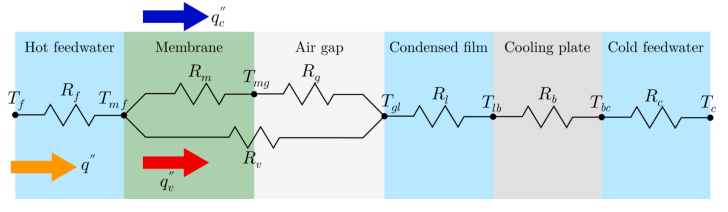
\includegraphics[width=0.5\linewidth]{Imagens//chap03/resistencias.png}
    \caption{}
    \label{fig:placeholder}
\end{figure}

As resistências condutivas consideradas no modelo correspondem à condução de calor através da membrana e do espaço de ar. Para a membrana, a resistência térmica condutiva é dada por:

\begin{equation}
R_m = \frac{\delta_m}{k_m}
\end{equation}

\noindent em que \(R_m\) é a resistência térmica condutiva da membrana, \(\delta_m\) é a espessura da membrana e \(k_m\) é a condutividade térmica da membrana.

Para o espaço de ar, a resistência térmica condutiva é expressa por:

\begin{equation}
R_g = \frac{\delta_g}{k_g}
\end{equation}

\noindent em que \(R_g\) é a resistência térmica condutiva do espaço de ar, \(\delta_g\) é a espessura do espaço de ar e \(k_g\) é a condutividade térmica do ar.

O calor latente associado ao transporte de vapor é expresso por

\begin{equation}
q_v'' = j_w h_{lv}
\end{equation}

em que $q_v''$ é o fluxo de calor latente ($\mathrm{W\,m^{-2}}$), $j_w$ é o fluxo mássico de permeado e $h_{lv}$ é o calor latente de vaporização da água.

A formulação adotada baseia-se em uma analogia com circuitos resistivos para representar os transportes de massa e calor. Nessa analogia, o fluxo é associado a uma força motriz e a uma resistência: para o transporte de massa, a força motriz é a diferença de pressão parcial de vapor; para o transporte de calor, é a diferença de temperatura entre as regiões do módulo.

No caso térmico, a utilização de uma resistência equivalente pressupõe regime estacionário, de modo que o fluxo de calor total seja constante ao longo das camadas consideradas. Nessas condições, as contribuições de convecção, condução e transporte de calor associado ao vapor podem ser representadas por resistências térmicas individuais, cuja combinação fornece uma resistência térmica equivalente para o sistema.

Assim, a resistência térmica equivalente do sistema pode ser escrita genericamente como:


\begin{equation}
R_{eq}
=
R_f +
\frac{R_v (R_m + R_g)}{R_v + R_m + R_g}
+ R_l + R_b + R_c
\end{equation}

\noindent sendo $R_v$, $R_l$ e $R_b$ resistências associadas aos mecanismos de transporte de vapor, condensação e condução estrutural.

O fluxo térmico total entre os canais quente e frio é então

\begin{equation}
q'' = \frac{T_f - T_c}{R_{eq}}
\end{equation}

onde $T_f$ e $T_c$ representam as temperaturas médias das correntes quente e fria.



\subsection{Indicadores de Desempenho Energético}

Além do fluxo de permeado, a avaliação de sistemas de destilação por membranas também pode envolver indicadores energéticos, uma vez que o processo depende do fornecimento de calor para promover a evaporação da água. Entre os indicadores utilizados na literatura estão o consumo específico de energia térmica (\textit{Specific Energy Consumption} -- SEC) e a razão de ganho de saída (\textit{Gain Output Ratio} -- GOR).

O consumo específico de energia térmica representa a quantidade de energia térmica fornecida ao sistema por unidade de volume de permeado produzido. Essa métrica pode ser expressa como a razão entre a taxa de calor externo fornecida ao sistema e a vazão volumétrica de permeado (\cite{curcino2023}):

\begin{equation}
SEC_{th} = \frac{\dot{Q}_{ext}}{\dot{V}_{w}}
\end{equation}

\noindent em que \(SEC_{th}\) é o consumo específico de energia térmica, \(\dot{Q}_{ext}\) é a taxa de calor externo fornecida ao sistema e \(\dot{V}_{w}\) é a vazão volumétrica de permeado produzido.

A razão de ganho de saída, por sua vez, relaciona o calor latente associado à produção de permeado com a energia térmica fornecida ao sistema. Esse indicador é frequentemente utilizado para avaliar o aproveitamento energético do processo, especialmente em sistemas com recuperação de calor:

\begin{equation}
GOR = \frac{\dot{V}_w \rho_w \Delta h_{lv}}{\dot{Q}_{ext}}
\end{equation}

\noindent em que \(GOR\) é a razão de ganho de saída, \(\rho_w\) é a massa específica da água e \(\Delta h_{lv}\) é o calor latente de vaporização.

\section{Modelo Físico Reduzido}

O presente trabalho utiliza como referência o modelo físico reduzido proposto por \cite{Lisboa2024}, desenvolvido para representar o comportamento global de um sistema V-AGMD em escala piloto. Nesta fundamentação teórica, o objetivo não é reproduzir integralmente a formulação apresentada no artigo, mas destacar os aspectos do modelo que são relevantes para a construção da abordagem metodológica adotada neste TCC.

O modelo é classificado como reduzido por representar o módulo por meio de parâmetros concentrados, sem resolver explicitamente perfis espaciais de temperatura, concentração, pressão ou velocidade ao longo dos canais. Dessa forma, o sistema é descrito a partir de grandezas médias ou efetivas, combinadas por balanços globais de massa e energia e por relações de transporte baseadas em resistências equivalentes.

No contexto deste trabalho, o modelo reduzido desempenha três funções principais. Primeiro, fornece uma referência físico-matemática para representar o comportamento esperado do sistema V-AGMD. Segundo, permite comparar as previsões obtidas por modelos orientados por dados com uma formulação baseada em princípios físicos. Terceiro, fornece informação física que pode ser incorporada às abordagens híbridas avaliadas posteriormente.

As principais grandezas estimadas pelo modelo incluem o fluxo de permeado e as temperaturas de saída das correntes do sistema. Essas variáveis são relevantes tanto para a avaliação da produtividade do processo quanto para o cálculo de indicadores energéticos. Assim, o modelo físico reduzido funciona como uma representação fenomenológica simplificada do sistema, conectando os mecanismos de transferência de massa e calor às variáveis de desempenho analisadas neste trabalho.

Por se tratar de uma formulação 0D, o modelo apresenta menor custo computacional quando comparado a modelos distribuídos. Essa característica é importante para sua utilização como referência em um pipeline de modelagem, pois permite gerar estimativas físicas de forma relativamente rápida, sem exigir a resolução detalhada dos campos espaciais no interior do módulo.

Entretanto, as simplificações adotadas também delimitam seu alcance. Como o modelo trabalha com grandezas médias, ele não representa explicitamente variações locais ao longo do módulo, como gradientes axiais de temperatura, concentração e velocidade. Além disso, fenômenos como polarização de concentração, efeitos hidrodinâmicos locais, fouling e alterações estruturais da membrana não são diretamente contemplados.

Dessa forma, neste TCC, o modelo reduzido não é tratado como uma descrição completa do sistema, mas como uma aproximação físico-matemática útil para incorporar conhecimento fenomenológico à modelagem. Suas previsões são utilizadas como referência e como fonte de informação física, sempre considerando as limitações associadas à formulação concentrada e às hipóteses simplificadoras adotadas.
\section{Aprendizado de Máquinas}

O Aprendizado de Máquina (\textit{Machine Learning}) constitui uma abordagem associada à Inteligência Artificial voltada ao desenvolvimento de modelos capazes de aprender a partir de dados observados, identificando padrões e relações que podem ser utilizados para realizar previsões a partir de novos exemplos (\cite{Ghahramani2015}). Diferentemente de modelos baseados em física ou equações, nos quais as relações entre variáveis são formuladas previamente a partir de conhecimento científico, leis de conservação e hipóteses teóricas, os modelos de aprendizado de máquina aprendem relações entrada-saída diretamente dos dados, ajustando seus parâmetros durante o treinamento para minimizar uma função de erro associada à tarefa de interesse (\cite{Rai2020}).

De forma geral, o objetivo do aprendizado de máquinas é estimar uma função que relacione um conjunto de variáveis de entrada a uma variável, ou variáveis, de saída.

Os métodos de aprendizado podem ser classificados em três categorias principais \cite{Sarkar2018PML}:

\begin{itemize}
    \item \textbf{Aprendizado supervisionado}: utiliza dados rotulados, ou seja, pares entrada–saída conhecidos. O modelo aprende uma função que mapeia as entradas nas saídas observadas. Problemas de regressão e classificação pertencem a essa categoria.
    
    \item \textbf{Aprendizado não supervisionado}: opera sobre dados sem rótulos explícitos, buscando identificar padrões estruturais, agrupamentos ou representações latentes.
    
    \item \textbf{Aprendizado por reforço}: baseia-se em interações sequenciais com o ambiente, onde decisões são tomadas visando maximizar uma recompensa acumulada.
\end{itemize}



Diversas técnicas foram desenvolvidas para tarefas supervisionadas, incluindo regressão linear, modelos regularizados, árvores de decisão, métodos baseados em \textit{ensembles} e redes neurais artificiais. Cada uma dessas abordagens apresenta características distintas quanto à complexidade, capacidade de generalização e interpretabilidade, aspectos que serão discutidos nas seções seguintes.

\subsection{Formulação do Problema de Regressão}

Em regressão supervisionada, assume-se que os dados observados são gerados a partir de um modelo estatístico da forma

\begin{equation}
Y = f(X) + \varepsilon,
\end{equation}

onde $X$ representa o vetor de variáveis de entrada, $Y$ é a variável resposta e $\varepsilon$ é um termo de erro aleatório tal que $E(\varepsilon)=0$ e $\varepsilon$ é independente de $X$ (\cite{Sarkar2018PML}). Nesse modelo, a função verdadeira $f(x)$ coincide com a média condicional:

\begin{equation}
f(x) = E(Y \mid X = x).
\end{equation}

O objetivo do aprendizado é estimar uma função \(\hat{f}\), a partir de um conjunto finito de observações \(\{(x_i, y_i)\}_{i=1}^{N}\), capaz de produzir boas previsões para novos valores de entrada dentro da faixa de operação coberta pelo conjunto de treinamento.

\subsubsection*{Perda Quadrática e Erro Esperado de Predição}

Para quantificar erros de predição, introduz-se uma função de perda $L(Y,f(X))$. A forma mais comum é a perda quadrática,

\begin{equation}
L(Y,f(X)) = (Y - f(X))^2.
\end{equation}

Sob essa escolha, define-se o erro esperado de predição (do inglês, \textit{Expected Prediction Error}) como

\begin{equation}
EPE(f) = E[(Y - f(X))^2],
\end{equation}

onde a expectativa é tomada sobre a distribuição conjunta de $(X,Y)$. Pode-se escrever equivalentemente

\begin{equation}
EPE(f) = E_X \, E_{Y|X} \left[(Y - f(X))^2 \mid X \right].
\end{equation}

A minimização do EPE pode ser realizada ponto a ponto em $x$, resultando em

\begin{equation}
f(x) = \arg\min_c E_{Y|X} \left[(Y - c)^2 \mid X = x \right].
\end{equation}

A solução desse problema é dada pela média condicional,

\begin{equation}
f(x) = E(Y \mid X = x),
\end{equation}

mostrando que, sob perda quadrática, a melhor predição possível é a média condicional da variável resposta.

\subsubsection*{Erro de Treinamento e Generalização}

Na prática, a distribuição verdadeira dos dados é desconhecida, de modo que o EPE não pode ser calculado diretamente. Em seu lugar, utiliza-se o erro de treinamento, definido pelo critério de soma de quadrados dos resíduos, definido por:

\begin{equation}
RSS(f) = \sum_{i=1}^{N} (y_i - f(x_i))^2.
\end{equation}

A minimização do $RSS$ produz um estimador ajustado aos dados observados. Entretanto, um modelo que apresenta erro de treinamento muito baixo pode não apresentar desempenho equivalente em novos pontos de teste. O erro esperado em novas observações — também chamado de erro de teste ou erro de generalização — corresponde ao EPE avaliado em dados independentes do conjunto de treinamento.

Essa distinção entre erro de treinamento e erro de teste é fundamental para a análise do desempenho preditivo e será explorada nas seções seguintes.

\subsection{Métricas de Avaliação para Regressão}

A avaliação do desempenho preditivo dos modelos de regressão é realizada por meio de funções de perda ou funções de pontuação (do inglês, \textit{scoring functions}), que quantificam a discrepância entre os valores observados $y_i$ e as previsões $\hat{y}_i$. 

As funções de pontuação são ferramentas padrão para avaliação de modelos, sendo exemplos clássicos o erro quadrático e o erro absoluto (\cite{Fissler2022ModelComparison}). No contexto deste trabalho, foram consideradas métricas amplamente utilizadas em problemas de regressão, uma vez que as variáveis de interesse, como fluxo de permeado e temperaturas de saída, são contínuas. Assim, o erro quadrático médio (MSE), a raiz do erro quadrático médio (RMSE), o erro absoluto médio (MAE), o erro percentual absoluto médio (MAPE) e o coeficiente de determinação (\(R^2\)) foram utilizados por fornecerem avaliações complementares do desempenho preditivo.

O MSE e o RMSE penalizam mais fortemente erros de maior magnitude, sendo úteis para identificar modelos com grandes desvios de previsão. O MAE fornece uma medida direta do erro médio absoluto, com menor sensibilidade a desvios extremos. O MAPE expressa o erro em termos relativos, permitindo interpretar o desvio percentual entre previsões e valores observados. Já o \(R^2\) avalia a proporção da variabilidade dos dados explicada pelo modelo. Dessa forma, a combinação dessas métricas permite analisar não apenas a magnitude dos erros, mas também a qualidade global do ajuste obtido pelos modelos.

\subsubsection{Erro Quadrático Médio (MSE)}

O erro quadrático médio ( do inglês, \textit{Mean Squared Error} -- MSE) mede a média dos quadrados das diferenças entre os valores observados e os valores previstos pelo modelo. Para um conjunto com \(N\) observações, essa métrica é definida como:

\begin{equation}
MSE = \frac{1}{N}\sum_{i=1}^{N}(y_i - \hat{y}_i)^2,
\end{equation}

\noindent em que \(y_i\) representa o valor observado da variável de saída para a amostra \(i\), \(\hat{y}_i\) representa o valor previsto pelo modelo para essa mesma amostra e \(N\) é o número total de observações.
\subsubsection*{Raiz do Erro Quadrático Médio (RMSE)}

A raiz do erro quadrático médio é definida como:

\begin{equation}
\mathrm{RMSE} = \sqrt{\mathrm{MSE}}.
\end{equation}

A aplicação da raiz quadrada constitui uma transformação monotônica, de modo que MSE e RMSE induzem a mesma ordenação de modelos. A principal vantagem do RMSE é expressar o erro na mesma unidade da variável resposta, facilitando sua interpretação física (\cite{Fissler2022ModelComparison}).

\subsubsection*{Erro Absoluto Médio (MAE)}

A função de perda absoluta é definida como:

\begin{equation}
L(z,y) = |z - y|.
\end{equation}

O erro absoluto médio (Mean Absolute Error, MAE) é dado por:

\begin{equation}
\mathrm{MAE} = \frac{1}{n} \sum_{i=1}^{n} |\hat{y}_i - y_i|.
\end{equation}

O erro absoluto é estritamente consistente para o funcional mediana condicional. Diferentemente do MSE, o MAE não eleva os erros ao quadrado, tornando-o menos sensível a valores extremos. Sua unidade coincide com a unidade da variável resposta (\cite{Fissler2022ModelComparison}).

\subsubsection*{Erro Percentual Absoluto Médio (MAPE)}

O erro percentual absoluto é definido como:

\begin{equation}
\mathrm{APE}_i = \left| \frac{y_i - \hat{y}_i}{y_i} \right|.
\end{equation}

O erro percentual absoluto médio (MAPE) é então:

\begin{equation}
\mathrm{MAPE} = \frac{1}{n} \sum_{i=1}^{n} 
\left| \frac{y_i - \hat{y}_i}{y_i} \right|.
\end{equation}

Essa métrica é adimensional, permitindo comparação relativa entre diferentes variáveis. Entretanto, apresenta limitações quando $y_i$ assume valores próximos de zero, podendo gerar instabilidades numéricas.

\subsubsection*{Coeficiente de Determinação ($R^2$)}

O coeficiente de determinação mede a proporção da variância da variável resposta explicada pelo modelo. Para um conjunto com $n$ observações, é definido por:

\begin{equation}
R^2 = 1 - 
\frac{\sum_{i=1}^{n}(y_i - \hat{y}_i)^2}
{\sum_{i=1}^{n}(y_i - \bar{y})^2},
\end{equation}

onde $\bar{y}$ representa a média amostral:

\begin{equation}
\bar{y} = \frac{1}{n}\sum_{i=1}^{n} y_i.
\end{equation}

O valor máximo de $R^2$ é 1, indicando ajuste perfeito. Valores negativos podem ocorrer quando o modelo apresenta desempenho inferior ao de um modelo constante que sempre prediz a média amostral.

O $R^2$ fornece uma medida de qualidade de ajuste baseada na variância explicada, sendo amplamente utilizado em problemas de regressão.

\subsection{Correlação, Associação Estatística e Causalidade}
\label{subsec:correlacao_associacao_causalidade}

A análise de correlação é uma ferramenta estatística utilizada para investigar a associação entre duas variáveis. No contexto deste trabalho, essa análise é empregada de forma exploratória, com o objetivo de identificar tendências gerais entre as variáveis operacionais de entrada e as variáveis de saída do sistema V-AGMD. Entretanto, diferentes coeficientes de correlação capturam diferentes tipos de associação, sendo importante distinguir suas interpretações.

O coeficiente de correlação de Pearson, usualmente representado por \(r\), é associado à análise de relações lineares entre duas variáveis quantitativas. Valores positivos indicam que as variáveis tendem a aumentar conjuntamente, enquanto valores negativos indicam que uma variável tende a diminuir quando a outra aumenta. Valores próximos de zero indicam ausência de associação linear forte, embora não excluam a possibilidade de relações não lineares. Dessa forma, o coeficiente de Pearson é mais adequado quando se deseja avaliar a presença de uma tendência aproximadamente linear entre as variáveis.

O coeficiente de correlação de Spearman, usualmente representado por \(\rho\), é calculado a partir dos postos, ou posições ordenadas, das observações. Por esse motivo, ele é frequentemente utilizado para avaliar associações monotônicas, isto é, situações em que uma variável tende a aumentar ou diminuir de forma consistente em relação à outra, ainda que a relação não seja necessariamente linear. Assim, Spearman pode ser mais apropriado em análises exploratórias nas quais se deseja identificar tendências crescentes ou decrescentes sem impor uma forma linear específica à relação entre as variáveis. (\cite{VanDenHeuvel2022Correlation})

Apesar dessa distinção, ambos os coeficientes devem ser interpretados como medidas de associação estatística. Eles indicam o grau e a direção de uma relação observada entre variáveis, mas não estabelecem, por si só, uma relação de causa e efeito. Como discutido por \cite{Holland1986StatisticsCausal}, correlação não implica causalidade: a observação de que duas variáveis variam conjuntamente não significa necessariamente que uma delas cause a outra. A associação observada pode decorrer de efeitos indiretos, de variáveis não consideradas, de restrições impostas pelo planejamento experimental ou da combinação simultânea de múltiplas condições operacionais.

Essa distinção é particularmente relevante porque as análises de dispersão e correlação são utilizadas como ferramentas exploratórias para apoiar a compreensão inicial dos dados. Assim, eventuais associações observadas entre variáveis de entrada e saída não são interpretadas como evidência causal isolada. As conclusões do estudo concentram-se na capacidade preditiva dos modelos avaliados e na identificação de padrões estatísticos dentro do domínio experimental analisado, sem assumir que as correlações observadas estabeleçam relações causais diretas entre as variáveis.

\subsubsection*{Considerações para Regressão Multi-Output}

No caso de regressão com múltiplas saídas, as métricas são calculadas individualmente para cada variável dependente. Essa abordagem permite avaliar o desempenho do modelo de forma específica para cada grandeza física prevista, evitando mascaramento de erros devido a diferenças de escala entre as variáveis.

Nas subseções seguintes, são apresentados o procedimento clássico de validação cruzada por \(K\) partições e a adaptação baseada em grupos, utilizada neste trabalho para respeitar a estrutura dos regimes operacionais.

\subsection{Controle de Complexidade e Overfitting}

O desempenho preditivo de um modelo supervisionado está diretamente relacionado ao seu grau de complexidade. Em problemas de regressão, assume-se tipicamente que os dados são gerados segundo

\begin{equation}
Y = f(X) + \varepsilon,
\end{equation}

onde $f(X)$ é a função verdadeira desconhecida e $\varepsilon$ é um termo de ruído com $E(\varepsilon)=0$ e $Var(\varepsilon)=\sigma_\varepsilon^2$. O objetivo do aprendizado é construir um estimador $\hat{f}(X)$ capaz de aproximar $f(X)$ a partir de um conjunto finito de dados. \cite{Hastie2009ESL}


\subsubsection{Complexidade do Modelo, Overfitting e Underfitting}

A flexibilidade de um modelo está associada à sua capacidade de se ajustar a diferentes formas funcionais entre as variáveis de entrada e a variável de saída. Modelos pouco flexíveis tendem a representar relações mais simples, enquanto modelos mais flexíveis conseguem capturar padrões mais complexos e não lineares nos dados. Entretanto, o aumento da flexibilidade também pode tornar o modelo mais sensível às particularidades do conjunto de treinamento, elevando o risco de \textit{overfitting} quando não há controle adequado de complexidade (\cite{Hastie2009ESL}).


Entretanto, essa maior flexibilidade pode levar ao fenômeno de \textit{overfitting}, no qual o modelo passa a capturar não apenas o padrão estrutural dos dados, mas também flutuações aleatórias específicas da amostra de treinamento. Nesse caso, o erro de treinamento tende a ser baixo, pois o modelo se ajusta muito bem aos dados utilizados no seu ajuste. No entanto, o erro de generalização pode ser elevado, uma vez que o modelo passa a ter dificuldade para realizar boas previsões em dados novos, não utilizados durante o treinamento. Assim, a diferença entre esses erros está no conjunto de dados considerado: o erro de treinamento é calculado sobre os dados usados para ajustar o modelo, enquanto o erro de generalização representa o desempenho esperado em novas observações.

Por outro lado, modelos excessivamente restritivos podem apresentar \textit{underfitting}, caracterizado por alto erro tanto no treinamento quanto na validação, devido à incapacidade de representar adequadamente a função subjacente.

Existe, portanto, um nível intermediário de complexidade que minimiza o erro esperado de predição.

\subsubsection{Decomposição Viés--Variância}

Sob perda quadrática, o erro esperado de predição em um ponto $x_0$ pode ser decomposto como

\begin{equation}
Err(x_0) = \sigma_\varepsilon^2 
+ \left[ E\hat{f}(x_0) - f(x_0) \right]^2 
+ E\left[ \hat{f}(x_0) - E\hat{f}(x_0) \right]^2.
\end{equation}

Os termos correspondem a:

\begin{itemize}
\item \textbf{Erro irredutível} ($\sigma_\varepsilon^2$): variabilidade inerente ao processo gerador dos dados;
\item \textbf{Viés ao quadrado}: erro sistemático introduzido pelas restrições do modelo;
\item \textbf{Variância}: sensibilidade do modelo às flutuações do conjunto de treinamento.
\end{itemize}

De modo geral, o aumento da complexidade reduz o viés, pois amplia o conjunto de funções representáveis, mas aumenta a variância, tornando o modelo mais sensível às particularidades da amostra. O erro total resulta do equilíbrio entre esses dois efeitos.


\subsubsection{Espaço do Modelo}

O espaço do modelo pode ser definido como o conjunto de todas as previsões possíveis que podem ser produzidas pelo procedimento de aprendizado. Modelos mais flexíveis possuem um espaço de hipóteses mais amplo, enquanto modelos mais restritivos operam em um subconjunto reduzido desse espaço.

A ampliação do espaço do modelo tende a reduzir o viés estrutural, porém aumenta a variabilidade das estimativas obtidas a partir de diferentes amostras.

\subsubsection{Regularização baseada em física}

A regularização é uma estratégia utilizada para controlar a complexidade do modelo e melhorar sua capacidade de generalização. Em termos gerais, ela consiste na introdução de penalizações associadas à complexidade ou à suavidade da função ajustada, restringindo a flexibilidade do modelo e reduzindo a tendência de ajuste excessivo aos dados de treinamento (\cite{Tian2022}).

Em modelos híbridos ou físico-informados, essa ideia pode ser estendida pela incorporação de termos associados ao conhecimento físico na função de perda. Nabian e Meidani propõem uma regularização orientada pela física na qual a função objetivo combina um termo de ajuste aos dados com um termo baseado no resíduo das equações governantes do sistema. Esse termo adicional penaliza desvios em relação às leis físicas conhecidas, induzindo o modelo a produzir soluções mais consistentes com o comportamento esperado do sistema (\cite{Nabian2020}).

Dessa forma, a regularização baseada em física pode ser interpretada como uma restrição adicional ao espaço de soluções admissíveis. Além de reduzir o erro em relação aos dados experimentais, o modelo passa a ser penalizado quando suas previsões violam relações físicas conhecidas. Essa estratégia é particularmente relevante em problemas com poucos dados rotulados ou com forte estrutura física subjacente, pois permite incorporar conhecimento fenomenológico ao treinamento e reduzir a ocorrência de previsões fisicamente inconsistentes (\cite{Nabian2020}).
\subsubsection{Graus de Liberdade Efetivos}

Em modelos gerais, a complexidade pode ser quantificada por meio dos graus de liberdade efetivos, que medem o grau de adaptação do modelo aos dados observados. Diferentemente do simples número de parâmetros, os graus de liberdade efetivos capturam a flexibilidade real do procedimento de ajuste, sendo aplicáveis também a métodos não paramétricos.

Essa noção fornece uma métrica unificada para comparar o nível de complexidade entre diferentes famílias de modelos.




\subsection{Validação Cruzada}
\label{sec:validacao_cruzada}

A avaliação de modelos supervisionados busca estimar sua capacidade de generalização, isto é, seu desempenho em observações não utilizadas durante o treinamento. De forma geral, esse desempenho pode ser associado ao erro esperado de predição extra-amostral. Conforme discutido em \cite{Hastie2009ESL}, esse erro pode ser expresso por

\begin{equation}
\mathrm{Err} = \mathbb{E}[L(Y,\hat{f}(X))],
\label{eq:erro_esperado_generalizacao}
\end{equation}

\noindent em que \(L(Y,\hat{f}(X))\) representa a função de perda entre o valor observado \(Y\) e a predição obtida pelo modelo \(\hat{f}(X)\). A expectativa é tomada sobre novas observações provenientes da mesma distribuição conjunta de \((X,Y)\).

Na prática, como a distribuição verdadeira dos dados é desconhecida, o erro de generalização não pode ser observado diretamente e precisa ser estimado a partir do conjunto de dados disponível. Assim, os procedimentos de validação buscam fornecer estimativas empíricas do desempenho preditivo esperado, permitindo comparar modelos, selecionar hiperparâmetros e avaliar a capacidade de generalização das soluções obtidas.

\subsubsection*{Divisão treino--teste}

Uma estratégia simples para estimar o desempenho de generalização é a divisão treino--teste, também associada à abordagem de validação por conjunto separado. Nesse procedimento, a base de dados é particionada em subconjuntos disjuntos, de modo que uma parte dos dados seja utilizada para o ajuste do modelo e outra parte seja reservada para avaliar seu desempenho em observações não empregadas no treinamento.

Em uma formulação mais completa, pode-se ainda separar os dados em três subconjuntos: treinamento, validação e teste. O conjunto de treinamento é utilizado para ajustar os parâmetros do modelo, o conjunto de validação auxilia na escolha de modelos ou hiperparâmetros, e o conjunto de teste deve ser reservado para a avaliação final do modelo selecionado. Como discutido por \cite{Hastie2009ESL}, o conjunto de teste deve ser mantido separado até o final da análise, pois seu uso repetido durante a seleção pode levar a uma estimativa excessivamente otimista do erro de generalização.

Apesar de sua simplicidade, essa estratégia pode ser limitada quando o número de observações disponíveis é reduzido. Nesses casos, a separação da base em múltiplos subconjuntos diminui a quantidade de dados disponível para o ajuste do modelo e pode tornar a avaliação sensível à composição dos subconjuntos utilizados. Por esse motivo, métodos baseados em reutilização eficiente da amostra, como a validação cruzada e o bootstrap, são frequentemente empregados em situações nas quais não há dados suficientes para uma divisão convencional em conjuntos de treinamento, validação e teste (\cite{Hastie2009ESL}).

\begin{figure}[H]
    \centering
    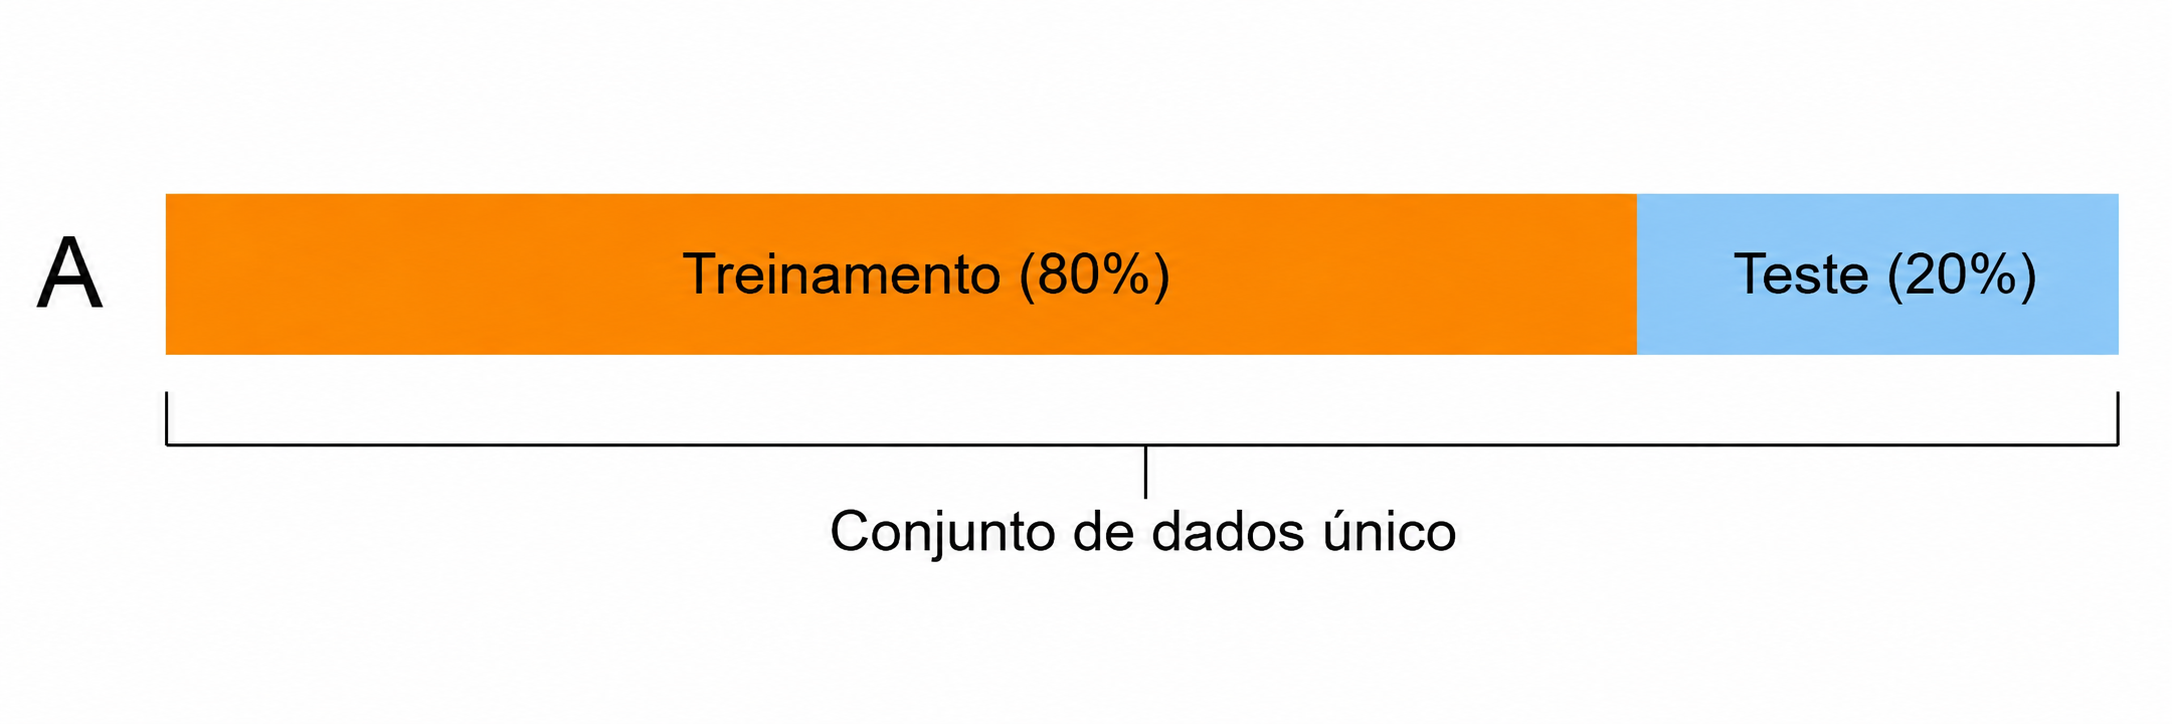
\includegraphics[width=0.75\linewidth]{Imagens/chap04/8020.png}
    \caption[Divisão treino--teste 80/20]{Representação esquemática da divisão treino--teste simples na proporção 80/20. Nessa estratégia, o conjunto de dados é separado uma única vez em dois subconjuntos: 80\% das observações são utilizadas para treinamento do modelo e 20\% são reservadas para avaliação do desempenho preditivo, sem serem utilizadas no ajuste dos parâmetros do modelo. Fonte: Elaborado pela autora.}
    \label{fig:divisao_treino_teste_80_20}
\end{figure}
\subsubsection*{Validação Cruzada \(K\)-Fold}

Na validação cruzada \(K\)-fold, o conjunto de dados é dividido em \(K\) subconjuntos aproximadamente do mesmo tamanho. Para cada partição \(k = 1, \dots, K\), o modelo é ajustado utilizando \(K-1\) subconjuntos, enquanto o subconjunto restante é utilizado para validação. O processo é repetido até que todos os subconjuntos tenham sido utilizados uma vez como conjunto de validação.

Formalmente, seja \(k(i)\) a função que indica a qual subconjunto pertence a observação \(i\), e seja \(\hat{f}^{-k(i)}\) o modelo ajustado excluindo o subconjunto \(k(i)\). A estimativa de validação cruzada é dada por

\begin{equation}
\mathrm{CV}(\hat{f}) =
\frac{1}{N}
\sum_{i=1}^{N}
L\big(y_i, \hat{f}^{-k(i)}(x_i)\big).
\label{eq:cv_estimativa}
\end{equation}

Quando o modelo depende de um hiperparâmetro \(\alpha\), a estimativa pode ser escrita como

\begin{equation}
\mathrm{CV}(\hat{f},\alpha) =
\frac{1}{N}
\sum_{i=1}^{N}
L\big(y_i, \hat{f}^{-k(i)}(x_i,\alpha)\big).
\label{eq:cv_hiperparametro}
\end{equation}

Nesse caso, o valor de \(\alpha\) que minimiza \(\mathrm{CV}(\hat{f},\alpha)\) pode ser selecionado, e o modelo final é então ajustado utilizando todos os dados disponíveis com esse hiperparâmetro. Valores usuais de \(K\) são 5 ou 10, representando um compromisso prático entre estabilidade da estimativa e custo computacional (\cite{Hastie2009ESL}).

\begin{figure}[H]
    \centering
    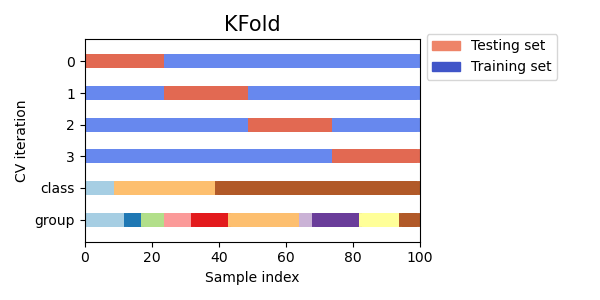
\includegraphics[width=0.75\linewidth]{Imagens/chap04/k-fold.png}
    \caption[Validação cruzada \(K\)-fold]{Representação esquemática da validação cruzada \(K\)-fold. O conjunto de dados é dividido em \(K\) partições e, a cada iteração, uma partição é utilizada para validação enquanto as demais são utilizadas para treinamento. Fonte: \cite{sklearn_groupkfold_docs}}
    \label{fig:kfold_validacao}
\end{figure}

\subsubsection*{Validação Cruzada Agrupada}

Em alguns conjuntos de dados, as observações não podem ser consideradas completamente independentes entre si. Isso ocorre, por exemplo, quando diferentes amostras pertencem a um mesmo grupo experimental, indivíduo, unidade de ensaio, condição operacional ou regime de operação. Nesses casos, uma validação cruzada aleatória pode distribuir observações correlacionadas simultaneamente entre treinamento e validação, produzindo estimativas excessivamente otimistas de desempenho.

Para lidar com essa limitação, pode-se utilizar a validação cruzada agrupada. Nessa estratégia, os grupos definidos pelo usuário são tratados como unidades indivisíveis durante o particionamento dos dados. Assim, todas as observações pertencentes a um mesmo grupo são alocadas integralmente no conjunto de treinamento ou no conjunto de validação em cada iteração. Esse procedimento permite avaliar a capacidade do modelo de generalizar para grupos não utilizados durante o ajuste, reduzindo o risco de que informações associadas a um mesmo grupo experimental estejam presentes simultaneamente nos subconjuntos de treinamento e validação.

% CITAÇÃO A VERIFICAR:
% A documentação do scikit-learn pode sustentar a descrição operacional do GroupKFold.
% Para fundamentação acadêmica, buscar uma fonte sobre grouped cross-validation,
% clustered data, repeated measurements ou dependência entre observações experimentais.

\begin{figure}[H]
    \centering
    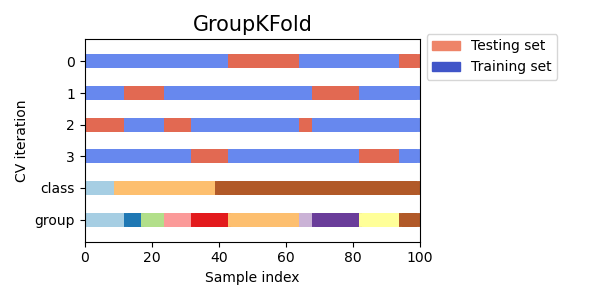
\includegraphics[width=0.75\linewidth]{Imagens/chap04/group_k_fold.png}
    \caption[Validação cruzada agrupada]{Representação esquemática da validação cruzada agrupada. Nesse procedimento, todas as observações pertencentes a um mesmo grupo experimental são mantidas na mesma partição, evitando que amostras correlacionadas sejam distribuídas simultaneamente entre treinamento e validação. Fonte: \cite{sklearn_groupkfold_docs}}
    \label{fig:groupkfold_validacao}
\end{figure}

\subsubsection*{Incerteza na Estimação do Desempenho Preditivo}

Embora a validação cruzada seja amplamente utilizada para estimar o desempenho preditivo de modelos, sua interpretação exige cuidado. A estimativa obtida por validação cruzada não deve ser entendida como uma medida exata do erro de predição do modelo final ajustado aos dados observados. Como discutido por \cite{Bates2022CV}, a validação cruzada estima, de forma mais adequada, o erro médio esperado de modelos ajustados a diferentes conjuntos de treinamento hipotéticos provenientes da mesma distribuição, e não necessariamente o erro específico do modelo ajustado à amostra disponível.

No contexto da validação cruzada com \(K\) partições, seja \(\mathcal{L}^{(k)}_{\mathrm{val}}\) a métrica de validação obtida na partição \(k\). A média das métricas de validação é dada por

\begin{equation}
\overline{\mathcal{L}}_{\mathrm{val}} =
\frac{1}{K}\sum_{k=1}^{K} \mathcal{L}^{(k)}_{\mathrm{val}}.
\label{eq:media_validacao}
\end{equation}

\noindent Essa média fornece uma estimativa pontual do desempenho preditivo esperado associado ao procedimento de modelagem avaliado. Entretanto, como as métricas podem variar entre as partições, é importante considerar também a dispersão dos resultados obtidos ao longo da validação cruzada. De forma prática, essa variabilidade pode ser resumida por meio do erro padrão:

\begin{equation}
\mathrm{SE}(\overline{\mathcal{L}}_{\mathrm{val}}) =
\frac{\sigma(\mathcal{L}_{\mathrm{val}})}{\sqrt{K}},
\label{eq:erro_padrao_validacao}
\end{equation}

\noindent em que \(\sigma(\mathcal{L}_{\mathrm{val}})\) representa o desvio padrão das métricas de validação obtidas nas \(K\) partições.

Essa medida, contudo, deve ser interpretada como uma aproximação prática da variabilidade observada entre partições, e não como uma caracterização exata da incerteza estatística do erro de generalização. Intervalos de confiança ingênuos derivados da validação cruzada podem apresentar cobertura inferior à nominal, pois estimativas de erro obtidas em diferentes partições não são completamente independentes, havendo correlação entre elas devido ao reaproveitamento dos dados nos processos de treinamento e validação \cite{Bates2022CV}. De forma complementar, \cite{BengioGrandvalet2003VarianceKFold} mostram que a estimação da variância do estimador de validação cruzada é um problema não trivial, não existindo estimador não viesado dessa variância a partir de uma única execução de validação cruzada.

O erro padrão calculado entre partições pode ser utilizado como uma medida prática da dispersão das métricas de validação, auxiliando a comparação entre modelos e a formulação de critérios de seleção que considerem a variabilidade da estimativa. Entretanto, essa medida deve ser interpretada com cautela: ela não corresponde a um intervalo de confiança exato para o desempenho real de generalização, mas a um indicador aproximado da variabilidade associada à avaliação em amostras finitas.


\subsubsection*{Sobreajuste no Processo de Seleção de Modelos}

A validação cruzada é frequentemente utilizada não apenas para estimar desempenho, mas também como critério de seleção de modelos, hiperparâmetros ou arquiteturas. Nesse caso, o processo de seleção passa a depender diretamente de uma estimativa de desempenho de generalização, como o erro médio obtido por validação cruzada. Como esse critério possui componentes de viés e variância, a escolha da configuração com menor erro médio pode favorecer modelos que apresentam desempenho aparentemente superior devido à variabilidade da estimativa, e não necessariamente por melhor capacidade real de generalização (\cite{Cawley2010Overfitting}).

Esse fenômeno é conhecido na literatura como sobreajuste no processo de seleção de modelos. Ele ocorre quando a otimização entre múltiplas configurações explora a variabilidade presente no critério de validação, selecionando uma alternativa que se ajusta excessivamente às particularidades da amostra ou das partições utilizadas na avaliação. Como consequência, o desempenho estimado para o modelo selecionado pode apresentar viés de seleção e viés otimista em relação ao desempenho esperado em dados verdadeiramente novos (\cite{Cawley2010Overfitting}).

Esse risco tende a ser mais pronunciado quando o conjunto de dados é pequeno, quando o critério de seleção apresenta variância não desprezível ou quando o número de hiperparâmetros a serem ajustados é relativamente grande. Nesses casos, a busca por configurações ótimas pode se tornar mais sensível às flutuações do critério de validação, aumentando a chance de selecionar uma configuração que parece superior na amostra analisada, mas que não necessariamente generaliza melhor (\cite{Cawley2010Overfitting}).

Para mitigar esse problema, a seleção de modelos deve ser tratada como parte integrante do próprio processo de ajuste do modelo, sendo refeita sempre que o procedimento for aplicado a uma nova amostra de dados. Essa perspectiva evita que a avaliação de desempenho desconsidere a variabilidade introduzida pela etapa de seleção e reduz o risco de estimativas excessivamente otimistas (\cite{Cawley2010Overfitting}).

Além disso, regras de seleção parcimoniosas podem ser utilizadas quando o objetivo é escolher uma configuração robusta, evitando favorecer modelos mais complexos cuja melhora de desempenho esteja dentro da incerteza da estimativa. Entre essas regras, destaca-se a regra do \textit{one-standard-error}, discutida a seguir.
% CITAÇÃO A VERIFICAR:
% Fonte sugerida: \cite{Hastie2009ESL}.
% Buscar também Yates2021Parsimonious ou Yates2023CV, caso sejam usadas
% para justificar seleção parcimoniosa considerando incerteza.
\subsubsection*{Seleção de Modelos pela Regra do \textit{One-Standard-Error}}

A regra do \textit{one-standard-error} é uma estratégia de seleção parcimoniosa baseada nas estimativas de validação cruzada. Em vez de escolher necessariamente o modelo com menor erro médio, esse critério seleciona o modelo mais simples cujo desempenho esteja dentro de uma margem de um erro padrão em relação ao melhor modelo observado. (\cite{Yates2022})

Para métricas de erro, identifica-se inicialmente o modelo \(m^\ast\) com menor erro médio de validação. Em seguida, considera-se elegível qualquer modelo \(m\) que satisfaça

\begin{equation}
\overline{\mathcal{L}}_{\mathrm{val}}(m)
\leq
\overline{\mathcal{L}}_{\mathrm{val}}(m^\ast)
+
\mathrm{SE}\left(\overline{\mathcal{L}}_{\mathrm{val}}(m^\ast)\right),
\label{eq:one_standard_error}
\end{equation}

\noindent em que \(m^\ast\) representa o modelo com menor erro médio de validação, \(\overline{\mathcal{L}}_{\mathrm{val}}(m^\ast)\) é esse menor erro médio, e \(m\) representa um modelo candidato cujo erro médio está dentro do limite de um erro padrão em relação ao melhor modelo.

Entre os modelos que satisfazem essa condição, seleciona-se aquele de menor complexidade. Dessa forma, a regra do \textit{one-standard-error} evita favorecer modelos mais complexos quando sua melhora de desempenho está dentro da variabilidade da estimativa de validação cruzada (\cite{Hastie2009ESL}).

A noção de menor complexidade depende da família de modelos considerada, podendo estar associada, por exemplo, à intensidade da regularização, à profundidade de árvores, ao número de estimadores, ao número de parâmetros ajustáveis ou ao tamanho de uma arquitetura neural. Portanto, a regra não define a complexidade de forma universal, mas estabelece um critério geral de seleção parcimoniosa a partir das estimativas de validação cruzada.
\subsection{Estratégias de Pré-processamento e Engenharia de Dados}

O desempenho de modelos de aprendizado supervisionado pode ser significativamente influenciado pelas etapas de pré-processamento e engenharia de atributos. O pré-processamento corresponde ao conjunto de procedimentos aplicados aos dados antes do treinamento, com o objetivo de padronizar escalas, reduzir inconsistências, tratar ruídos ou adequar as variáveis ao algoritmo utilizado. Já a engenharia de atributos envolve a transformação, seleção ou construção de variáveis de entrada, buscando representar melhor as informações relevantes para o processo de modelagem.

Nesta seção, são apresentadas algumas ferramentas de tratamento e preparação dos dados utilizadas ou avaliadas neste trabalho, incluindo discretização de variáveis contínuas, escalonamento, seleção de atributos e geração sintética de dados. Essas técnicas podem contribuir para melhorar a estabilidade numérica dos modelos, reduzir redundâncias, capturar relações não lineares e favorecer a capacidade de generalização.

\subsubsection{Binning (Discretização de Variáveis Contínuas)}

O \textit{binning}, também denominado discretização ou quantização, consiste na transformação de variáveis numéricas contínuas em variáveis discretas por meio da divisão de seu domínio em intervalos (bins). Cada intervalo representa uma faixa de valores e recebe um rótulo ou código discreto.

Conforme descrito em \cite{Sarkar2018PML}, a discretização pode ser realizada por meio de esquemas de largura fixa ( do inglês, \textit{fixed-width binning}) ou por estratégias adaptativas, como discretização baseada em quantis, nas quais os limites dos intervalos são definidos com base na própria distribuição dos dados.

Formalmente, dada uma variável contínua \(x \in \mathbb{R}\), define-se uma partição do seu domínio em \(K\) intervalos disjuntos:
\[
I_1, I_2, \dots, I_K,
\]
tal que
\[
\bigcup_{k=1}^{K} I_k = \mathrm{dom}(x)
\quad \text{e} \quad
I_i \cap I_j = \emptyset \ \text{para} \ i \neq j.
\]

\noindent em que \(x\) representa a variável contínua a ser discretizada, \(\mathbb{R}\) representa o conjunto dos números reais, \(K\) é o número total de intervalos definidos, \(I_k\) representa o \(k\)-ésimo intervalo da partição, \(\mathrm{dom}(x)\) é o domínio da variável \(x\), e \(I_i \cap I_j = \emptyset\) indica que os intervalos são disjuntos, isto é, não possuem elementos em comum quando \(i \neq j\).

Cada observação \(x\) é então mapeada para o índice do intervalo ao qual pertence.

A discretização pode ser particularmente útil quando a variável contínua apresenta distribuição assimétrica, caudas longas ou concentração de observações em determinadas faixas de valores. Nesses casos, a transformação em intervalos pode facilitar a representação da estrutura dos dados, reduzindo a influência de variações muito pequenas dentro de uma mesma faixa. Além disso, essa técnica pode ser empregada quando se deseja capturar relações não lineares de forma simplificada, especialmente em modelos que se beneficiam de representações por faixas em vez de relações estritamente contínuas ou lineares.

\paragraph{Risco de perda de informação}

Apesar de suas possíveis vantagens, a discretização implica em perda de informação. Ao substituir um valor contínuo por um identificador de intervalo, elimina-se a variação interna dentro de cada bin.

Esse processo pode:

\begin{itemize}
    \item Reduzir a resolução da variável;
    \item Introduzir descontinuidades artificiais;
    \item Aumentar a dimensionalidade quando utilizada codificação categórica;
    \item Gerar instabilidade caso os limites dos bins não possuam fundamentação estatística ou física.
\end{itemize}

Assim, a aplicação de binning deve ser cuidadosamente avaliada, considerando tanto seus potenciais ganhos de modelagem quanto os riscos associados à perda de granularidade dos dados.

\subsubsection{Padronização e Escalonamento de Variáveis}

Em problemas de aprendizado de máquina envolvendo variáveis numéricas contínuas, é comum que diferentes atributos apresentem ordens de grandeza significativamente distintas. Algumas variáveis podem assumir valores muito elevados, enquanto outras permanecem em faixas reduzidas. O uso direto dessas variáveis pode introduzir viés numérico no processo de treinamento, favorecendo atributos com maior magnitude.

Conforme discutido em \cite{Sarkar2018PML}, muitos algoritmos são sensíveis à escala dos dados, especialmente modelos lineares e métodos baseados em otimização gradiente-dependente. Dessa forma, técnicas de escalonamento de variáveis (do inglês, \textit{feature scaling}) são frequentemente empregadas para transformar os atributos para uma escala comum.

\paragraph{Padronização}

No presente trabalho, a padronização é relevante porque as variáveis de entrada do sistema V-AGMD possuem unidades físicas e ordens de grandeza distintas, como temperatura, vazão, pressão de vácuo e concentração salina. A padronização por \textit{Z-score} consiste em centralizar cada variável em torno de sua média e escalá-la pelo desvio padrão, de modo que as variáveis transformadas apresentem média nula e desvio padrão unitário. Essa transformação coloca as variáveis em uma escala numérica comparável, evitando que diferenças arbitrárias de unidade ou magnitude influenciem de forma desproporcional o ajuste dos modelos. Esse cuidado é particularmente importante em modelos regularizados, nos quais a penalização dos coeficientes pode ser afetada pela escala das variáveis de entrada (\cite{James2013ISL}).

Matematicamente, a transformação é dada por:

\begin{equation}
X' = \frac{X - \mu_X}{\sigma_X},
\label{eq:padronizacao_zscore}
\end{equation}

\noindent em que \(X\) representa a variável original, \(\mu_X\) é sua média, \(\sigma_X\) é seu desvio padrão e \(X'\) é a variável padronizada.

\paragraph{Normalização Min-Max}

O escalonamento Min-Max transforma os valores da variável para um intervalo fixo, geralmente \([0,1]\). A transformação é definida como:

\begin{equation}
X' = \frac{X - \min(X)}{\max(X) - \min(X)}.
\label{eq:normalizacao_minmax}
\end{equation}

\noindent em que \(X\) representa a variável original, \(\min(X)\) e \(\max(X)\) representam, respectivamente, os valores mínimo e máximo dessa variável no conjunto de dados, e \(X'\) representa a variável normalizada.

Esse método preserva a forma da distribuição original, mas comprime os dados dentro de um intervalo limitado. Entretanto, é sensível à presença de outliers, pois valores extremos afetam diretamente os limites da transformação.

\paragraph{Robust Scaling}

Para mitigar a influência de valores extremos, pode-se utilizar o escalonamento robusto, baseado em estatísticas menos sensíveis a outliers. Nesse caso, a transformação é definida como:

\begin{equation}
X' = \frac{X - \mathrm{median}(X)}{IQR(X)},
\label{eq:robust_scaling}
\end{equation}

\noindent em que \(\mathrm{median}(X)\) representa a mediana da variável e \(IQR(X)\) representa o intervalo interquartil, definido como a diferença entre o terceiro e o primeiro quartil.

Essa abordagem reduz o impacto de observações extremas e pode ser mais adequada quando a distribuição apresenta caudas longas ou assimetria significativa.

\paragraph{Sensibilidade dos Modelos à Escala}

Nem todos os modelos apresentam a mesma sensibilidade à escala das variáveis. Modelos baseados em distâncias e métodos lineares regularizados são particularmente afetados por diferenças de magnitude entre atributos. Quando variáveis possuem escalas muito distintas, aquelas com valores numericamente maiores tendem a exercer maior influência no processo de otimização.

\paragraph{Impacto em Redes Neurais e Regressões Regularizadas}

O escalonamento é especialmente importante em:

\begin{itemize}
    \item \textbf{Redes neurais}: a ausência de padronização pode levar a gradientes instáveis e dificultar a convergência do treinamento. Dados centralizados e com variância controlada contribuem para uma superfície de otimização mais bem condicionada.

    \item \textbf{Regressões regularizadas (Ridge, Lasso, ElasticNet)}: como a penalização é aplicada diretamente sobre os coeficientes, diferenças de escala entre variáveis podem resultar em penalizações desbalanceadas. A padronização assegura que a regularização atue de forma equitativa entre os atributos.
\end{itemize}

Dessa forma, o escalonamento constitui etapa fundamental do pipeline de pré-processamento em modelos sensíveis à magnitude das variáveis, sendo prática recomendada quando se utilizam métodos lineares regularizados ou redes neurais (\cite{Sarkar2018PML}).
\subsubsection{Seleção de Atributos}

Em problemas de aprendizado supervisionado, os atributos correspondem às variáveis de entrada utilizadas pelo modelo para realizar previsões. No contexto deste trabalho, esses atributos representam as condições operacionais do sistema V-AGMD, como temperaturas de entrada, vazão, pressão de vácuo e concentração salina. A escolha adequada dessas variáveis é importante porque elas determinam quais informações estarão disponíveis para que o modelo aprenda a relação com as saídas de interesse.

A utilização de um grande número de atributos pode aumentar a complexidade do modelo, elevar o risco de sobreajuste (\textit{overfitting}) e dificultar a interpretação dos resultados. Nesse contexto, a seleção de atributos (\textit{feature selection}) tem como objetivo identificar um subconjunto relevante de variáveis de entrada que contribua para melhorar o desempenho preditivo e a capacidade de generalização do modelo (\cite{Sarkar2018PML}).

As estratégias de seleção de atributos podem ser agrupadas em três categorias principais:

As estratégias de seleção de atributos podem ser agrupadas em três categorias principais:

\paragraph{Filter Methods}

Os métodos do tipo filtro selecionam atributos com base em métricas estatísticas independentes de qualquer modelo específico. Exemplos incluem medidas de correlação, informação mútua e testes estatísticos. Esses métodos avaliam a relação individual entre cada atributo e a variável resposta, sem envolver o treinamento de modelos preditivos.

\paragraph{Wrapper Methods}

Os métodos do tipo \textit{wrapper} utilizam um modelo preditivo como parte do processo de seleção. Nesse caso, diferentes subconjuntos de atributos são avaliados por meio do treinamento e validação de modelos, sendo selecionado aquele que apresenta melhor desempenho. Estratégias sequenciais comuns incluem a seleção \textit{forward} e a eliminação \textit{backward}. 

Na seleção \textit{forward}, o procedimento se inicia sem atributos no modelo e, a cada etapa, adiciona-se a variável que mais melhora o critério de desempenho adotado. Na eliminação \textit{backward}, o procedimento parte do conjunto completo de atributos e remove, a cada etapa, a variável cuja retirada menos prejudica ou mais melhora o desempenho do modelo. Em ambos os casos, os subconjuntos candidatos são avaliados iterativamente com base em um critério definido, como erro de validação ou critérios de informação, até que se obtenha uma combinação considerada adequada (\cite{Hastie2009ESL}).


\paragraph{Embedded Methods}

Os métodos embarcados (\textit{embedded}) integram o processo de seleção ao próprio treinamento do modelo. Algoritmos baseados em árvores e métodos de ensemble são exemplos típicos, pois incorporam mecanismos internos de avaliação da importância das variáveis.

\paragraph{Benefícios da Seleção de Atributos}

A seleção de atributos pode proporcionar:

\begin{itemize}
    \item Melhor desempenho preditivo;
    \item Redução do risco de sobreajuste;
    \item Modelos mais simples e interpretáveis;
    \item Redução do custo computacional.
\end{itemize}

Assim, a seleção de atributos constitui etapa relevante no pipeline de engenharia de dados, especialmente em cenários com múltiplas variáveis candidatas e possível redundância entre elas.

\subsection{Famílias de Modelos}
\subsubsection{Regressão Linear e Modelos Regularizados}

A regressão linear é um dos métodos mais fundamentais em aprendizado supervisionado para modelagem de relações entre variáveis de entrada e uma resposta contínua. Dados \(n\) exemplos de treinamento \(\{(x_i, y_i)\}_{i=1}^n\), com \(x_i \in \mathbb{R}^p\) e \(y_i \in \mathbb{R}\), objetivamos aprender uma função linear da forma

\begin{equation}
\hat{y} = w_0 + \sum_{j=1}^{p} w_j x_j,
\end{equation}

onde \(w_0\) é o termo de intercepto e \(w_j\) são os coeficientes associados às variáveis preditoras. A escolha dos coeficientes é baseada na minimização de uma função de custo, tipicamente o erro quadrático médio entre as previsões \(\hat{y}_i\) e os valores observados \(y_i\).

\subsubsection{Regressão Linear Ordinária (OLS)}

Na regressão linear ordinária (do inglês, \textit{Ordinary Least Squares -- OLS}), busca-se o vetor de coeficientes
\(\mathbf{w}\) que minimiza a soma dos quadrados dos resíduos, isto é,
\begin{equation}
\hat{\mathbf{w}}
=
\arg\min_{\mathbf{w}}
\|\mathbf{X}\mathbf{w} - \mathbf{y}\|_2^2.
\end{equation}

A Figura~\ref{fig:reg_ols} ilustra, de forma simplificada, o ajuste de uma regressão linear por mínimos quadrados ordinários. Os pontos representam observações do conjunto de dados, enquanto a reta corresponde à função linear estimada pelo modelo. A comparação entre os painéis de treino e teste permite visualizar que o modelo ajustado busca capturar uma tendência média dos dados, mas sua capacidade preditiva deve ser avaliada também em observações não utilizadas no ajuste.

\begin{figure}[H]
    \centering
    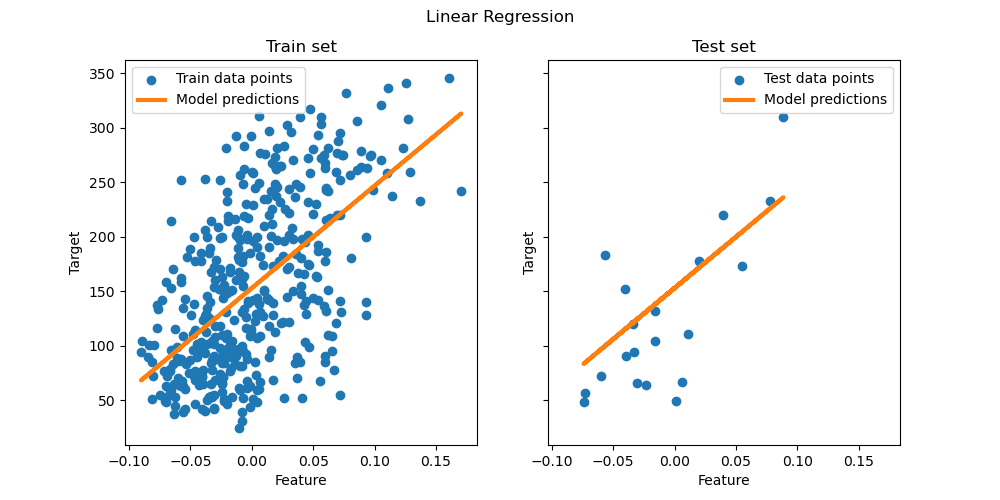
\includegraphics[width=0.75\linewidth]{Imagens/chap02/reg_OLS.png}
    \caption[Exemplo de regressão linear OLS]{Exemplo de regressão linear pelo método dos mínimos quadrados ordinários (OLS).}
    \fonte{\cite{sklearn_groupkfold_docs}}
    \label{fig:reg_ols}
\end{figure}

Os estimadores de mínimos quadrados dependem fortemente da independência linear entre as colunas da matriz de projeto \(\mathbf{X}\). Quando existe correlação elevada entre preditores — situação conhecida como multicolinearidade — a matriz \(\mathbf{X}^T \mathbf{X}\) pode tornar-se próxima de singular. Como consequência, a solução dos mínimos quadrados torna-se numericamente instável e altamente sensível a pequenas variações nos dados, produzindo estimativas com grande variância (\cite{scikit-learn-linear-model}). 

Esse fenômeno compromete a capacidade de generalização do modelo e motiva o uso de modelos lineares regularizados. Conforme discutido anteriormente, a regularização atua como um mecanismo de controle de complexidade, restringindo a flexibilidade do modelo e reduzindo sua sensibilidade às particularidades do conjunto de treinamento. Nesta seção, essa ideia é retomada no contexto específico dos modelos lineares, por meio das regressões Ridge e Lasso, apresentadas a seguir.

\subsubsection{Regressão Regularizada}

A regularização é uma técnica que penaliza a complexidade do modelo para melhorar sua capacidade de generalização e mitigar problemas como multicolinearidade ou sobreajuste (overfitting). Modelos regularizados adicionam termos de penalização à função de custo.

\paragraph{Ridge Regression (Penalização L2)}

A regressão Ridge surge como uma extensão da regressão linear ordinária com o objetivo de mitigar problemas associados à multicolinearidade e à elevada variância das estimativas. O método introduz uma penalização quadrática sobre os coeficientes do modelo, modificando o problema de otimização para

\begin{equation}
\hat{\mathbf{w}}
=
\arg\min_{\mathbf{w}}
\left(
\|\mathbf{X}\mathbf{w} - \mathbf{y}\|_2^2
+
\alpha \|\mathbf{w}\|_2^2
\right),
\end{equation}

onde \(\alpha \ge 0\) é o parâmetro de regularização.


\medskip

O termo adicional \(\alpha \|\mathbf{w}\|_2^2\) impõe uma penalização proporcional ao quadrado da magnitude dos coeficientes. À medida que \(\alpha\) aumenta, maior é o encolhimento (shrinkage) aplicado aos parâmetros do modelo, reduzindo sua magnitude e tornando a solução mais robusta à colinearidade entre variáveis explicativas.

O parâmetro \(\alpha\) controla diretamente o compromisso entre ajuste aos dados e complexidade do modelo. Para \(\alpha = 0\), recupera-se a solução de mínimos quadrados ordinários. Para valores crescentes de \(\alpha\), os coeficientes são progressivamente reduzidos em magnitude, o que diminui a variância do estimador, ainda que introduza um viés adicional.

Esse comportamento ilustra o clássico compromisso viés-variância: o aumento da regularização tende a reduzir a sensibilidade do modelo a flutuações nos dados de treinamento, melhorando potencialmente sua capacidade de generalização.

\paragraph{Lasso Regression (Penalização L1)}

A Lasso (Least Absolute Shrinkage and Selection Operator) é um modelo linear regularizado que introduz uma penalização baseada na norma L1 dos coeficientes. Diferentemente da Ridge regression, cuja penalização é quadrática, a Lasso impõe uma penalização linear sobre a magnitude absoluta dos parâmetros, favorecendo soluções esparsas.

O problema de otimização associado pode ser escrito como

\begin{equation}
\hat{\mathbf{w}}
=
\arg\min_{\mathbf{w}}
\left(
\frac{1}{2n}
\|\mathbf{X}\mathbf{w} - \mathbf{y}\|_2^2
+
\alpha \|\mathbf{w}\|_1
\right),
\end{equation}

onde
\(
\|\mathbf{w}\|_1 = \sum_{j=1}^{p} |w_j|
\)
e \(\alpha \ge 0\) controla a intensidade da regularização.

A principal característica da penalização \(L_1\) é sua capacidade de produzir coeficientes exatamente nulos. Como consequência, a Lasso pode realizar seleção implícita de variáveis, reduzindo o número efetivo de preditores utilizados pelo modelo.

Essa propriedade pode ser vantajosa quando há muitas variáveis candidatas ou quando se deseja obter um modelo mais simples e interpretável, pois variáveis com coeficientes nulos deixam de contribuir para a predição. No entanto, essa característica também deve ser interpretada com cuidado: em bases de dados pequenas ou com variáveis correlacionadas, a Lasso pode selecionar apenas uma entre variáveis com informações semelhantes, o que pode afetar a estabilidade da seleção.

Assim, Lasso é relevante não apenas como modelo de regressão regularizado, mas também como uma alternativa capaz de reduzir a complexidade do modelo por meio da exclusão automática de variáveis pouco informativas.

Assim como em outros modelos regularizados, o parâmetro \(\alpha\) controla o compromisso entre ajuste aos dados e complexidade do modelo. Valores elevados de \(\alpha\) aumentam a esparsidade e o viés do estimador, enquanto valores reduzidos aproximam a solução do estimador de mínimos quadrados ordinários.

\paragraph{Elastic Net}

O método Elastic Net combina as penalizações L1 e L2 em um único modelo linear regularizado. Seu objetivo é integrar a capacidade de seleção de variáveis da Lasso com a estabilidade numérica da Ridge, especialmente em cenários onde há correlação entre preditores.

O problema de otimização pode ser formulado como

\begin{equation}
\hat{\mathbf{w}}
=
\arg\min_{\mathbf{w}}
\left(
\frac{1}{2n}
\|\mathbf{X}\mathbf{w} - \mathbf{y}\|_2^2
+
\alpha
\left(
\rho \|\mathbf{w}\|_1
+
\frac{1-\rho}{2}
\|\mathbf{w}\|_2^2
\right)
\right),
\end{equation}

onde \(\alpha \ge 0\) controla a intensidade global da regularização e
\(\rho \in [0,1]\) determina o balanço entre as penalizações L1 e L2.

O parâmetro \(\rho\) define a combinação convexa entre as duas penalizações. Para \(\rho = 1\), o modelo reduz-se à Lasso; para \(\rho = 0\), torna-se equivalente à Ridge. Valores intermediários produzem um compromisso entre esparsidade e estabilidade.

O parâmetro \(\alpha\), por sua vez, controla o grau total de regularização aplicado ao modelo.

Em situações nas quais múltiplas variáveis apresentam forte correlação entre si, a Lasso tende a selecionar apenas uma delas, descartando as demais. O Elastic Net, ao incorporar o termo L2, tende a selecionar conjuntamente variáveis correlacionadas, distribuindo os coeficientes entre elas.

Essa propriedade torna o método particularmente útil em problemas com grupos de preditores correlacionados.

Outra vantagem prática do Elastic Net é sua maior estabilidade sob transformações lineares das variáveis de entrada. A presença da penalização L2 contribui para reduzir a sensibilidade da solução a pequenas perturbações nos dados, característica herdada da regressão Ridge.

Assim, o Elastic Net pode ser interpretado como uma generalização que engloba tanto a Lasso quanto a Ridge como casos particulares. Ele oferece maior flexibilidade na modelagem do compromisso entre viés, variância e esparsidade estrutural.


\subsubsection{Árvores de Decisão}

Árvores de Decisão (Decision Trees -- DTs) são métodos supervisionados não paramétricos utilizados para classificação e regressão. O objetivo é criar um modelo que prediga o valor de uma variável alvo por meio da aprendizagem de regras de decisão simples inferidas a partir dos atributos dos dados. Uma árvore pode ser vista como uma aproximação constante por partes.

Quanto maior a profundidade da árvore, mais complexas se tornam as regras de decisão e mais ajustado o modelo tende a ficar.

\begin{table}[H]
\centering
\caption[Vantagens e limitações das árvores de decisão]{Vantagens e limitações das árvores de decisão.}
\label{tab:vantagens_desvantagens_arvores}
\begin{tabular}{p{6.5cm} p{7.5cm}}
\hline
\textbf{Vantagens} & \textbf{Limitações} \\
\hline

São modelos de fácil interpretação, pois a estrutura da árvore permite visualizar as regras de decisão utilizadas para gerar as previsões. 
&
Podem apresentar \textit{overfitting} quando a árvore cresce excessivamente, ajustando-se a detalhes específicos do conjunto de treinamento e perdendo capacidade de generalização. \\

Exigem menor preparação prévia dos dados em comparação com outros métodos, pois não dependem diretamente de padronização das variáveis. 
&
São modelos instáveis, uma vez que pequenas alterações nos dados podem gerar árvores com estruturas bastante diferentes. \\

Podem capturar relações não lineares e interações entre variáveis sem a necessidade de especificar previamente a forma funcional da relação entre entradas e saída. 
&
Produzem previsões constantes por partes, o que pode limitar sua capacidade de representar relações suaves e comprometer sua aplicação em extrapolação. \\

Podem ser aplicadas tanto a problemas de classificação quanto de regressão, incluindo situações com múltiplas saídas, dependendo da implementação utilizada. 
&
A construção da árvore ótima é computacionalmente difícil; por isso, os algoritmos práticos utilizam estratégias heurísticas, que não garantem uma solução globalmente ótima. \\

Apresentam boa transparência em comparação com modelos do tipo \textit{black box}, como redes neurais, facilitando a análise das regras utilizadas pelo modelo. 
&
Podem apresentar viés quando há desbalanceamento nos dados ou quando determinadas regiões do espaço de entrada são pouco representadas. \\

\hline
\end{tabular}
\fonte{Adaptado de \cite{sklearn_groupkfold_docs}.}
\end{table}

A Figura~\ref{fig:arvore_decisao} ilustra o comportamento de uma árvore de decisão aplicada a um problema de regressão. Diferentemente de modelos lineares, que ajustam uma função contínua aos dados, a árvore de decisão aproxima a relação entre entrada e saída por regiões constantes por partes. A figura também permite observar o efeito da profundidade máxima da árvore sobre a complexidade do modelo: árvores mais rasas produzem aproximações mais simples, enquanto árvores mais profundas conseguem se ajustar mais detalhadamente aos dados.

\begin{figure}[H]
    \centering
    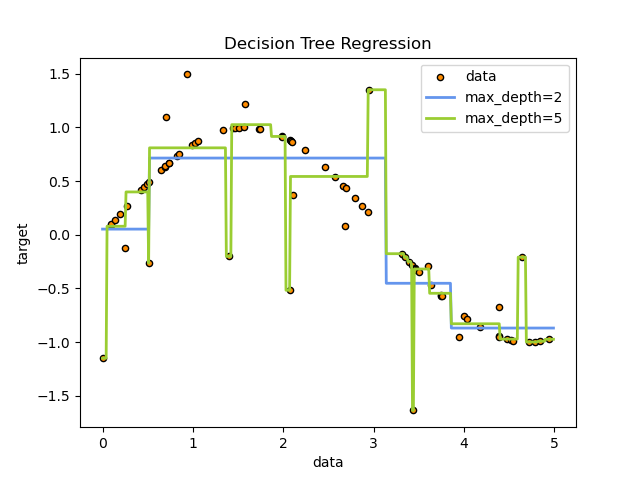
\includegraphics[width=0.5\linewidth]{Imagens/chap02/arvore.png}
    \caption[Regressão por árvore de decisão]{Exemplo de regressão utilizando árvore de decisão com diferentes profundidades, ilustrando o impacto da complexidade do modelo na capacidade de ajuste aos dados. Fonte: \cite{sklearn_groupkfold_docs}}
    \label{fig:arvore_decisao}
\end{figure}

Na Figura~\ref{fig:arvore_decisao}, a árvore com menor profundidade apresenta uma aproximação mais suave e simplificada da tendência geral dos dados. Já a árvore com maior profundidade acompanha variações mais locais, produzindo uma função mais irregular. Esse comportamento ilustra o compromisso entre flexibilidade e capacidade de generalização: o aumento da profundidade pode reduzir o erro no conjunto de treinamento, mas também aumenta o risco de \textit{overfitting}, caso o modelo passe a capturar flutuações específicas da amostra em vez do padrão geral dos dados.
\paragraph{Formulação Matemática}

Dados vetores de treinamento \(x_i \in \mathbb{R}^n\), \(i = 1, \dots, l\), e um vetor de rótulos \(y \in \mathbb{R}^l\), uma árvore de decisão particiona recursivamente o espaço de atributos de modo que amostras com os mesmos rótulos ou valores-alvo semelhantes sejam agrupadas.

Sejam os dados no nó \(m\) representados por \(Q_m\), contendo \(n_m\) amostras. Para cada divisão candidata \(\theta = (j, t_m)\), composta por um atributo \(j\) e um limiar \(t_m\), os dados são particionados em dois subconjuntos. O subconjunto à esquerda reúne as observações cujo valor do atributo \(j\) é menor ou igual ao limiar \(t_m\):

\begin{equation}
Q_m^{\mathrm{left}}(\theta) =
\{(x,y)\,|\, x_j \leq t_m\}.
\label{eq:subconjunto_esquerda_arvore}
\end{equation}

\noindent O subconjunto à direita é formado pelas demais observações do nó \(m\), isto é:

\begin{equation}
Q_m^{\mathrm{right}}(\theta) =
Q_m \setminus Q_m^{\mathrm{left}}(\theta).
\label{eq:subconjunto_direita_arvore}
\end{equation}

\noindent em que \(Q_m^{\mathrm{left}}(\theta)\) e \(Q_m^{\mathrm{right}}(\theta)\) representam, respectivamente, os subconjuntos resultantes da divisão à esquerda e à direita, \(x_j\) é o valor do atributo \(j\), \(t_m\) é o limiar de divisão no nó \(m\), e \(\setminus\) indica a diferença entre conjuntos.

A qualidade de uma divisão candidata no nó \(m\) é avaliada por meio de uma função de impureza ou função de perda \(H(\cdot)\), cuja escolha depende da tarefa considerada, como classificação ou regressão. Essa qualidade pode ser expressa por:

\begin{equation}
G(Q_m,\theta) =
\frac{n_m^{\mathrm{left}}}{n_m} H\left(Q_m^{\mathrm{left}}(\theta)\right)
+
\frac{n_m^{\mathrm{right}}}{n_m} H\left(Q_m^{\mathrm{right}}(\theta)\right).
\label{eq:criterio_divisao_arvore}
\end{equation}

\noindent em que \(G(Q_m,\theta)\) representa o valor do critério associado à divisão candidata \(\theta\) no nó \(m\), \(Q_m\) é o conjunto de amostras presentes nesse nó, \(n_m\) é o número total de amostras em \(Q_m\), \(Q_m^{\mathrm{left}}(\theta)\) e \(Q_m^{\mathrm{right}}(\theta)\) são os subconjuntos resultantes da divisão, e \(n_m^{\mathrm{left}}\) e \(n_m^{\mathrm{right}}\) representam o número de amostras em cada subconjunto. A função \(H(\cdot)\) mede a impureza ou erro associado a cada subconjunto.

A divisão ótima é então obtida pela escolha da divisão candidata que minimiza o critério \(G(Q_m,\theta)\):

\begin{equation}
\theta^* = \arg\min_{\theta} G(Q_m,\theta).
\label{eq:divisao_otima_arvore}
\end{equation}

\noindent em que \(\theta^*\) representa a melhor divisão encontrada para o nó \(m\), segundo o critério de impureza ou perda adotado.

A escolha da divisão em cada nó pode seguir diferentes estratégias. Uma estratégia baseada em busca exaustiva seleciona o par atributo--limiar que minimiza exatamente \(G(Q_m,\theta)\), avaliando todos os atributos disponíveis e todos os limiares possíveis. Alternativamente, pode-se utilizar uma estratégia aleatória, na qual um limiar candidato é amostrado aleatoriamente para cada atributo, resultando em uma aproximação estocástica da busca exaustiva e reduzindo o custo computacional.

Após selecionar a divisão ótima \(\theta^*\) no nó \(m\), o procedimento é aplicado recursivamente aos subconjuntos \(Q_m^{\mathrm{left}}(\theta^*)\) e \(Q_m^{\mathrm{right}}(\theta^*)\) até que uma condição de parada seja satisfeita, como profundidade máxima da árvore, número mínimo de amostras no nó ou redução mínima de impureza.

As árvores de decisão apresentam características que as tornam atrativas em problemas de regressão, especialmente pela facilidade de interpretação e pela capacidade de representar relações não lineares entre as variáveis. Entretanto, essas vantagens vêm acompanhadas de limitações importantes, principalmente relacionadas à instabilidade do modelo e ao risco de sobreajuste. A Tabela~\ref{tab:vantagens_desvantagens_arvores} resume os principais pontos positivos e negativos associados a esse tipo de modelo.
\subsubsection{Métodos de Combinação de Modelos (Ensemble Methods)}

Métodos de combinação de modelos (ensemble methods) consistem na estratégia de combinar as predições de múltiplos estimadores base, construídos a partir de um mesmo algoritmo de aprendizado, com o objetivo de melhorar a capacidade de generalização e a robustez do modelo final em comparação com um único estimador isolado.

Dois exemplos amplamente utilizados dessa abordagem são as Florestas Aleatórias (Random Forests) e o Gradient Boosting com Árvores de Decisão.

\subsubsection{Gradient Boosting com Árvores de Decisão}

O \textit{boosting} é um método de combinação de modelos no qual múltiplos estimadores simples, também chamados de \textit{weak learners}, são ajustados de forma sequencial para formar um modelo preditivo mais robusto. A ideia central é que cada novo estimador seja treinado buscando reduzir os erros remanescentes do modelo acumulado até a etapa anterior, de modo que a predição final resulte da combinação aditiva dos estimadores ajustados ao longo das iterações (\cite{Friedman2000}).

O \textit{Gradient Boosting} generaliza essa lógica ao formular o ajuste sequencial como uma descida do gradiente no espaço de funções. Nesse caso, a cada iteração, um novo estimador é ajustado na direção do gradiente negativo de uma função de perda diferenciável, permitindo aplicar o método a diferentes problemas supervisionados, incluindo regressão e classificação (\cite{Friedman2001}).


Modelos de \textit{Gradient Boosting} são modelos aditivos. A predição para uma entrada \(x_i\) é dada por:

Modelos de Gradient Boosting são modelos aditivos. A predição para uma entrada \( x_i \) é dada por

\[
\hat{y}_i = F_M(x_i) = \sum_{m=1}^{M} h_m(x_i),
\]

onde \( h_m \) são estimadores base, frequentemente chamados de \textit{weak learners} no contexto de boosting. No caso do Gradient Boosting com Árvores, esses estimadores base são árvores de decisão de tamanho fixo. O número total de árvores é denotado por \( M \).

O modelo é construído de forma sequencial e aditiva, por meio de um procedimento de otimização etapa a etapa, no qual cada novo estimador é ajustado para reduzir a função de perda considerando o modelo acumulado até a iteração anterior.

\[
F_m(x) = F_{m-1}(x) + h_m(x),
\]

onde cada nova árvore \( h_m \) é ajustada para minimizar uma função de perda acumulada:

\[
h_m = \arg\min_{h} \sum_{i=1}^{n} L\big(y_i, F_{m-1}(x_i) + h(x_i)\big),
\]

sendo  \(L(\cdot)\) uma função de perda diferenciável.

O modelo inicial \(F_0\) é escolhido como a constante que minimiza a função de perda antes da adição dos estimadores sequenciais. No caso da perda quadrática, tem-se:

\begin{equation}
F_0 = \arg\min_c \sum_{i=1}^{n} (y_i - c)^2.
\end{equation}

\noindent A solução desse problema é a média empírica dos valores alvo, isto é:

\begin{equation}
F_0 = \bar{y}.
\end{equation}

\noindent Assim, o modelo parte de uma predição inicial simples, correspondente à média dos valores observados, que é progressivamente corrigida pelos estimadores adicionados nas etapas seguintes.

Utilizando uma aproximação de Taylor de primeira ordem, pode-se demonstrar que, a cada iteração, a nova árvore \( h_m \) é ajustada para aproximar o gradiente negativo da função de perda em relação às predições atuais. Denotando

\[
g_i = \left[ \frac{\partial l(y_i, F(x_i))}{\partial F(x_i)} \right]_{F = F_{m-1}},
\]

a otimização se reduz, desprezando termos constantes, a

\[
h_m \approx \arg\min_{h} \sum_{i=1}^{n} h(x_i) g_i.
\]

Assim, a cada iteração, o estimador base é ajustado para prever o gradiente negativo da função de perda. Esse procedimento pode ser interpretado como uma forma de descida do gradiente em um espaço funcional.

\subsubsection{Controle da Complexidade das Árvores}

O tamanho das árvores de regressão utilizadas como estimadores base determina o nível de interação entre variáveis que o modelo pode capturar. Em geral, uma árvore de profundidade \( h \) pode capturar interações de ordem \( h \).

Existem duas formas principais de controlar o tamanho das árvores:

\begin{itemize}
\item Limitando a profundidade máxima da árvore, o que resulta em árvores binárias completas com até \( 2^h \) folhas e \( 2^h - 1 \) nós internos;
\item Limitando o número máximo de folhas, caso em que as árvores são construídas priorizando as divisões que produzem maior redução de impureza.
\end{itemize}

O controle do número de folhas define diretamente o grau máximo de interação modelável, sendo que uma árvore com \( k \) folhas possui \( k - 1 \) nós de divisão.

Em problemas com grande número de amostras, versões baseadas em histogramas podem apresentar ganhos significativos de eficiência computacional, além de oferecer suporte nativo a dados categóricos e valores ausentes. Em contrapartida, em conjuntos de dados pequenos, versões tradicionais podem ser preferíveis, pois a discretização por histogramas pode produzir pontos de divisão excessivamente aproximados.


\subsubsection{Random Forests e Outros Conjuntos de Árvores Aleatorizadas}

O conjunto de métodos de combinação de modelos (\textit{ensemble}) inclui algoritmos baseados na média de árvores de decisão aleatorizadas, como o \textit{Random Forest} e o método \textit{Extra-Trees}. Ambos seguem uma estratégia de perturbação e combinação ( do inglês, \textit{perturb-and-combine}), na qual diferentes árvores são construídas introduzindo variações nos dados de treinamento ou no processo de divisão dos nós. As previsões produzidas pelas árvores individuais são então combinadas, geralmente por meio de média, resultando em uma predição final mais robusta e menos sensível às particularidades de uma única árvore.

Assim como outros classificadores, modelos baseados em florestas são ajustados a partir de um conjunto de amostras de treinamento \(X \in \mathbb{R}^{n_{\text{samples}} \times n_{\text{features}}}\) e de um vetor de alvos \(Y \in \mathbb{R}^{n_{\text{samples}}}\). De forma análoga às árvores de decisão individuais, florestas também podem ser estendidas para problemas de múltiplas saídas.

\subsubsection{Random Forest}

Em Random Forests, cada árvore do conjunto é construída a partir de uma amostra obtida com reposição (\textit{bootstrap}) do conjunto de treinamento.

Durante a construção de cada árvore, um subconjunto aleatório das variáveis de entrada é considerado em cada divisão. O tamanho desse subconjunto pode incluir todas as variáveis ou apenas uma fração delas. 

Essas duas fontes de aleatoriedade — a amostragem com reposição das amostras e a seleção aleatória de variáveis em cada divisão — têm como objetivo reduzir a variância do estimador. Árvores de decisão individuais tendem a apresentar alta variância e, consequentemente, podem sofrer de sobreajuste. A aleatoriedade introduzida na floresta produz árvores com erros parcialmente desacoplados. Ao calcular a média das predições dessas árvores, parte desses erros pode se cancelar, reduzindo a variância global do modelo, possivelmente ao custo de um pequeno aumento no viés. Na prática, a redução de variância costuma ser significativa, resultando em melhor desempenho geral.

Durante o crescimento de cada árvore na floresta, a melhor divisão é escolhida de acordo com o critério de impureza, de maneira equivalente ao procedimento padrão utilizado em árvores de decisão do tipo CART. No caso de regressão, cada árvore produz uma previsão contínua para a variável de saída, e a previsão final da floresta é obtida pela média das previsões individuais. Essa combinação reduz a dependência em relação a uma única árvore e tende a diminuir a variância do modelo, tornando a predição mais robusta frente a pequenas variações no conjunto de treinamento.





\subsubsection{Perceptron Multicamadas (Multi-Layer Perceptron)}

O Perceptron Multicamadas (MLP) é um algoritmo de aprendizado supervisionado que aprende uma função 
\begin{equation}
f: \mathbb{R}^{m} \rightarrow \mathbb{R}^{o},
\label{eq:mlp_mapeamento}
\end{equation}
a partir de um conjunto de dados, onde \( m \) representa o número de dimensões de entrada e \( o \) o número de dimensões de saída. 

Dado um conjunto de atributos \( X = \{x_1, x_2, \dots, x_m\} \) e um alvo \( y \), o MLP é capaz de aprender um aproximador não linear da função de mapeamento, podendo ser aplicado tanto em problemas de classificação quanto de regressão. Diferentemente da regressão logística, o MLP possui uma ou mais camadas intermediárias não lineares entre a camada de entrada e a camada de saída, denominadas camadas ocultas.

A camada de entrada é composta por neurônios que representam diretamente os atributos de entrada. Cada neurônio em uma camada oculta realiza uma combinação linear ponderada das saídas da camada anterior,

\begin{equation}
w_1 x_1 + w_2 x_2 + \dots + w_m x_m
\end{equation}


seguida da aplicação de uma função de ativação não linear \( g(\cdot) : \mathbb{R} \rightarrow \mathbb{R} \), como, por exemplo, a tangente hiperbólica. A camada de saída recebe as ativações da última camada oculta e as transforma nos valores finais do modelo.

O modelo é parametrizado por matrizes de pesos que conectam camadas consecutivas e por vetores de bias associados a cada camada (exceto a camada de entrada). Cada matriz de pesos define as conexões entre duas camadas adjacentes, enquanto cada vetor de bias é somado às ativações lineares antes da aplicação da função de ativação.

\subsubsection{Algoritmos de Treinamento do MLP}

O MLP pode ser treinado utilizando diferentes algoritmos de otimização, como Gradiente Descendente Estocástico (SGD), Adam ou L-BFGS.

No caso do Gradiente Descendente Estocástico, os parâmetros são atualizados com base no gradiente da função de perda em relação aos pesos:

\[
w \leftarrow w - \eta \left[
\alpha \frac{\partial R(w)}{\partial w}
+
\frac{\partial \text{L}}{\partial w}
\right],
\]

onde \( \eta \) é a taxa de aprendizado, responsável por controlar o tamanho do passo na busca no espaço de parâmetros, \( \text{L} \) é a função de perda utilizada e \( R(w) \) representa um termo de regularização.

O método Adam também é um otimizador estocástico, porém ajusta automaticamente o tamanho das atualizações com base em estimativas adaptativas dos momentos de primeira e segunda ordem dos gradientes. Essa característica tende a favorecer a estabilidade do treinamento e a tornar o método menos sensível à escolha inicial da taxa de aprendizado.

Quando se utilizam métodos como SGD ou Adam, o treinamento pode ser realizado de forma \textit{online} ou por meio de mini-lotes. Isso permite atualizar os parâmetros a partir de subconjuntos dos dados, o que é vantajoso em bases maiores e em redes neurais treinadas iterativamente. Por outro lado, esses métodos podem exigir maior número de épocas e são sensíveis à escolha de hiperparâmetros, como taxa de aprendizado, tamanho do lote e critérios de parada.

O método L-BFGS, por sua vez, é um solucionador baseado em aproximações da matriz Hessiana, que representa as derivadas parciais de segunda ordem da função objetivo. Ele utiliza uma aproximação da inversa da Hessiana para atualizar os parâmetros, podendo apresentar convergência eficiente em problemas de menor dimensão ou com conjuntos de dados menores. Entretanto, diferentemente dos métodos baseados em gradiente estocástico, o L-BFGS não é adequado para aprendizado \textit{online} ou por mini-lotes, pois utiliza o conjunto de dados de forma mais global em cada atualização. Assim, sua aplicação pode se tornar menos prática em bases grandes, embora possa ser competitiva em problemas menores e bem condicionados.


\subsubsection{Vantagens e Limitações do MLP}

O Perceptron Multicamadas apresenta características que o tornam adequado para problemas de regressão não linear, como a capacidade de aproximar relações complexas entre variáveis de entrada e saída. Entretanto, essa flexibilidade também traz desafios relacionados ao treinamento, à escolha de hiperparâmetros e à sensibilidade ao pré-processamento dos dados. A Tabela~\ref{tab:vantagens_limitacoes_mlp} resume as principais vantagens e limitações associadas ao uso desse modelo.

\begin{table}[H]
\centering
\caption[Vantagens e limitações do Perceptron Multicamadas]{Vantagens e limitações do Perceptron Multicamadas.}
\label{tab:vantagens_limitacoes_mlp}
\begin{tabular}{p{6.5cm} p{7.5cm}}
\hline
\textbf{Vantagens} & \textbf{Limitações} \\
\hline

Capacidade de representar relações não lineares entre as variáveis de entrada e as saídas do modelo, o que torna o MLP adequado para problemas em que a relação entre as grandezas não pode ser descrita de forma simples ou linear.
&
A presença de camadas ocultas e funções de ativação não lineares torna a função de perda não convexa, podendo levar a diferentes soluções dependendo da inicialização dos pesos e do processo de treinamento. \\

Possibilidade de aprendizado incremental ou por mini-lotes, quando suportado pelo algoritmo de otimização utilizado, permitindo o ajuste iterativo dos parâmetros durante o treinamento.
&
O desempenho do modelo depende da escolha de diversos hiperparâmetros, como número de camadas ocultas, número de neurônios, função de ativação, taxa de aprendizado, regularização e critério de parada. \\

Capacidade de modelar interações complexas entre os atributos de entrada, sem exigir a especificação prévia da forma funcional da relação entre entradas e saídas.
&
O modelo é sensível à escala das variáveis de entrada, sendo recomendada a padronização prévia dos dados para evitar que diferenças de magnitude entre os atributos prejudiquem o treinamento. \\

\hline
\end{tabular}
\fonte{Adaptado de \cite{Sarkar2018PML}.}
\end{table}
\subsection{Modelos híbridos físico-informados e regularização baseada em física}
\label{sec:modelos-hibridos}

Em diversos problemas de engenharia, modelos puramente orientados a dados podem apresentar limitações importantes, especialmente em regimes com poucos dados rotulados e com forte estrutura física subjacente. Nesse contexto, abordagens híbridas buscam integrar conhecimento físico e aprendizado de máquina para induzir soluções mais plausíveis, consistentes e potencialmente mais robustas fora da distribuição de treinamento.

\subsubsection{Taxonomia de abordagens híbridas}
\label{subsec:taxonomia-hibrida}

Neste contexto, a taxonomia de abordagens híbridas refere-se a uma forma de classificar os diferentes modos pelos quais o conhecimento físico pode ser incorporado a modelos de aprendizado de máquina. Essa classificação é útil porque nem todas as abordagens híbridas combinam física e dados da mesma maneira: em alguns casos, a informação física é utilizada antes do treinamento, em outros é incorporada diretamente à estrutura do modelo e, em outros, aparece como restrição ou penalização na função de perda.

De acordo com \cite{rai2020hybrid}, as abordagens híbridas podem ser organizadas em três classes principais: (i) pré-processamento baseado em física, (ii) fusão na arquitetura do modelo de aprendizado de máquina e (iii) regularização baseada em física. A primeira classe abrange estratégias em que princípios físicos, modelos mecanísticos ou conhecimento externo são utilizados para transformar ou enriquecer as variáveis de entrada. A segunda classe refere-se a arquiteturas que incorporam explicitamente componentes físicos ou estruturais à rede. Já a terceira classe inclui métodos em que leis físicas, equações governantes ou relações conhecidas do sistema são incorporadas como restrições ou penalizações no processo de otimização, geralmente por meio de termos adicionais na função de perda.

A Figura~\ref{fig:taxonomia_hibrida_rai} apresenta essa classificação de forma esquemática. Nela, observa-se que o conhecimento físico pode ser incorporado em três momentos distintos do processo de modelagem. No primeiro caso, a física atua antes do treinamento, por meio do enriquecimento ou transformação das variáveis de entrada. No segundo, o conhecimento físico é incorporado à própria arquitetura do modelo, influenciando a forma como a rede neural processa as informações. No terceiro, a física é introduzida na função objetivo, penalizando soluções que se afastem de restrições, leis ou relações físicas conhecidas.

Essa representação é relevante para este trabalho porque permite situar as estratégias híbridas avaliadas posteriormente, especialmente aquelas em que a informação proveniente do modelo físico reduzido é utilizada como entrada adicional ou como termo de regularização durante o treinamento.

\begin{figure}[H]
    \centering
    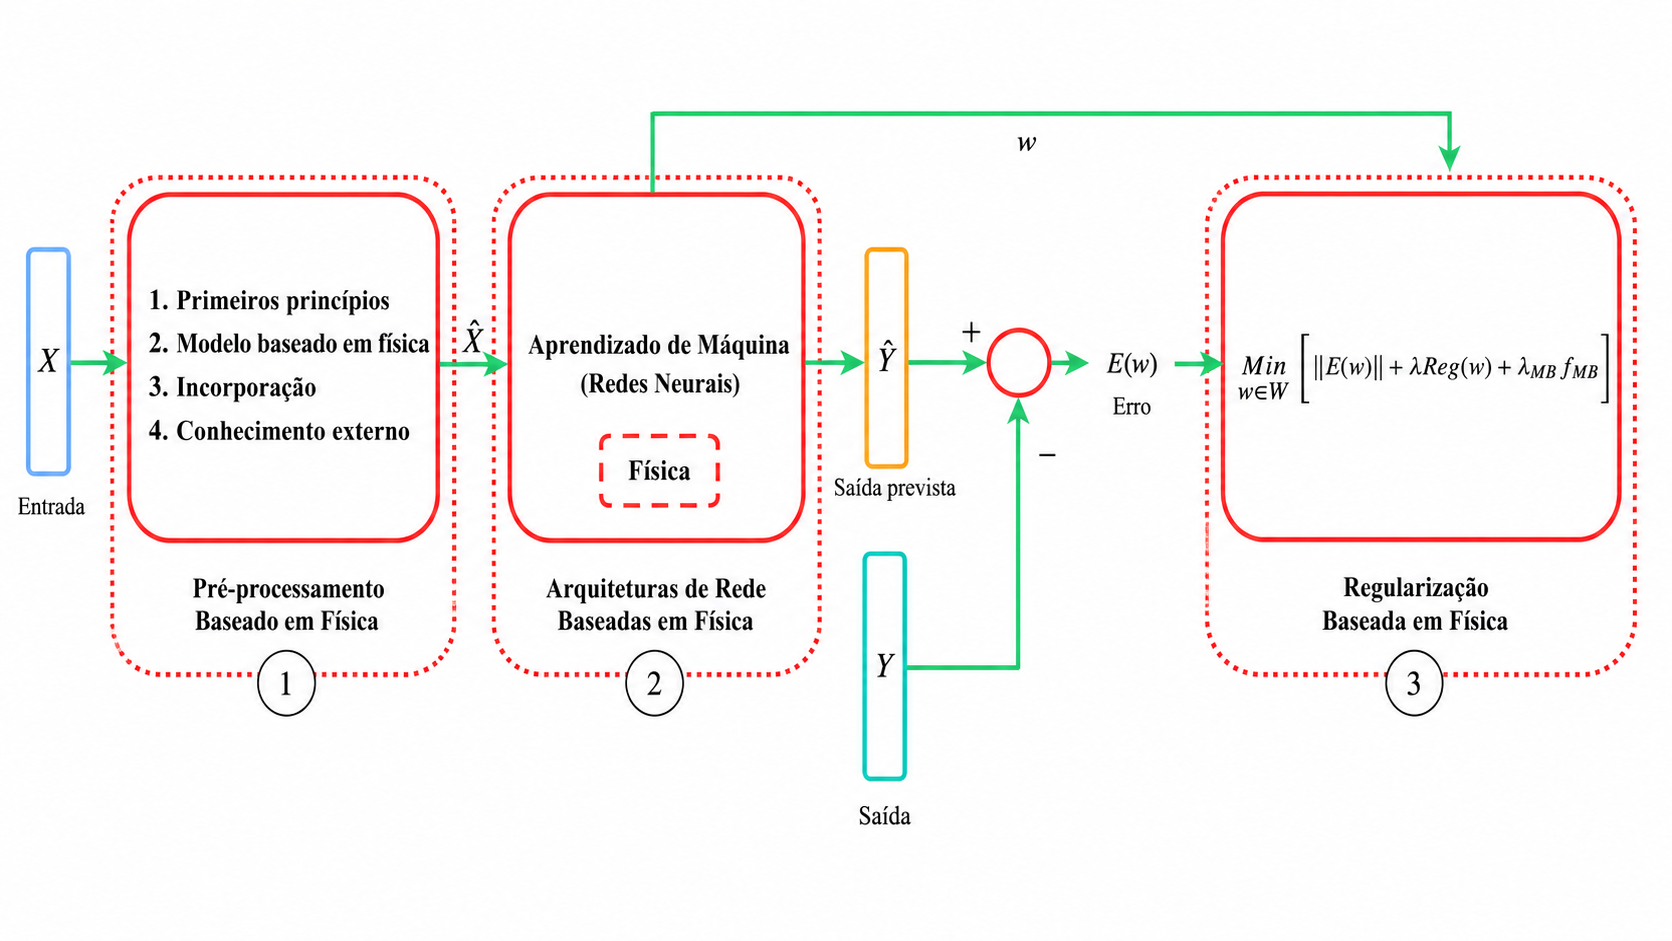
\includegraphics[width=0.95\linewidth]{Imagens/chap02/hybrid_tech.png}
    \caption[Taxonomia de abordagens híbridas guiadas por física]{Taxonomia de abordagens híbridas guiadas por física, classificadas em três categorias principais: (i) pré-processamento baseado em conhecimento físico, (ii) integração da física na arquitetura de redes neurais e (iii) incorporação de termos físicos na função de custo por meio de regularização.}
    \fonte{Adaptado de \cite{rai2020hybrid}.}
    \label{fig:taxonomia_hibrida_rai}
\end{figure}
\subsubsection{Regularização baseada em física via função de perda}

Uma formulação geral para tornar modelos de aprendizado de máquina mais consistentes com leis físicas consiste em acrescentar à função objetivo um termo adicional que penaliza violações de restrições físicas conhecidas do sistema. Nessa abordagem, a função de perda total passa a combinar três contribuições: (i) um termo de ajuste aos dados experimentais, que mede o erro entre valores observados e previstos; (ii) um termo de regularização clássica, associado ao controle da complexidade do modelo; e (iii) um termo de perda física, que quantifica o quanto as previsões do modelo desrespeitam leis físicas, equações governantes ou relações conhecidas do processo. De forma representativa, essa função pode ser escrita como \cite{willard2020}:

\begin{equation}
\mathcal{L} = \mathcal{L}_{\mathrm{TRN}}(\mathbf{Y}_{\mathrm{true}}, \mathbf{Y}_{\mathrm{pred}})
+ \lambda \,\mathcal{R}(\mathbf{W})
+ \gamma \,\mathcal{L}_{\mathrm{PHY}}(\mathbf{Y}_{\mathrm{pred}}),
\label{eq:loss_physics_based}
\end{equation}

\noindent em que $\mathcal{L}_{\mathrm{TRN}}(\mathbf{Y}_{\mathrm{true}}, \mathbf{Y}_{\mathrm{pred}})$ é o termo de ajuste aos dados de treinamento, normalmente definido por uma métrica de erro entre valores observados e previstos, como o erro quadrático médio; $\mathcal{R}(\mathbf{W})$ é o termo de regularização aplicado aos parâmetros do modelo $\mathbf{W}$, com o objetivo de controlar sua complexidade; e $\mathcal{L}_{\mathrm{PHY}}(\mathbf{Y}_{\mathrm{pred}})$ é o termo de perda física, responsável por penalizar previsões que violem relações físicas previamente conhecidas. Os parâmetros $\lambda$ e $\gamma$ controlam, respectivamente, a contribuição da regularização clássica e da restrição física na função objetivo total.

Do ponto de vista conceitual, a regularização física pode ser entendida como um mecanismo que restringe o conjunto de soluções admissíveis, impondo coerência com princípios físicos e reduzindo a dependência exclusiva de dados rotulados. Ao introduzir restrições físicas no processo de otimização, o espaço efetivo de busca para os parâmetros do modelo é reduzido, o que pode favorecer o aprendizado em regimes de poucos dados e incentivar previsões fisicamente consistentes.

É importante distinguir essa estratégia de uma \textit{Physics-Informed Neural Network} (PINN) em sentido estrito. Em uma PINN, as equações governantes do sistema, normalmente equações diferenciais ordinárias ou parciais, são incorporadas diretamente à função de perda por meio dos resíduos dessas equações. Assim, a rede é treinada não apenas para ajustar dados observados, mas também para satisfazer localmente as equações físicas no domínio considerado.

Na regularização física no nível da saída, por outro lado, a física não é necessariamente incorporada por meio do resíduo diferencial das equações governantes. Em vez disso, as previsões do modelo são comparadas com relações físicas conhecidas, restrições fenomenológicas ou saídas fornecidas por um modelo físico de referência. Dessa forma, o termo físico atua como uma penalização adicional sobre as saídas previstas, orientando o modelo a produzir respostas compatíveis com uma descrição física simplificada do sistema.


\subsubsection{Arquiteturas de redes baseadas em física}
\label{subsec:arquiteturas_fisicas}

Outra forma de integração entre conhecimento físico e modelos de
aprendizado de máquina consiste na incorporação explícita de
informações provenientes de modelos fenomenológicos na própria
arquitetura da rede neural. Nesse tipo de abordagem, o modelo físico
não atua apenas como uma fonte externa de informação, mas passa a
compor diretamente a estrutura do modelo híbrido.

De maneira geral, essa integração pode ocorrer de diferentes formas.
Uma possibilidade consiste em utilizar as predições de um modelo
físico como variáveis adicionais de entrada para a rede neural,
permitindo que o modelo baseado em dados explore diretamente a
informação fornecida pela modelagem fenomenológica. Alternativamente,
a rede neural pode ser estruturada para aprender o resíduo entre as
predições do modelo físico e os valores observados experimentalmente,
atuando como um mecanismo de correção sistemática das limitações do
modelo fenomenológico.

Essas estratégias caracterizam arquiteturas híbridas nas quais o
modelo físico e o modelo orientado a dados são acoplados de forma
estrutural. Nesse contexto, o modelo físico pode fornecer estimativas
iniciais, variáveis intermediárias ou componentes da própria função
de mapeamento aprendida pela rede neural, enquanto o modelo de
aprendizado de máquina captura efeitos não representados ou
aproximados na formulação física original.

Exemplos de arquiteturas desse tipo incluem modelos híbridos baseados
em dados físicos (\textit{hybrid physics data}), modelos de correção
residual e arquiteturas híbridas que combinam ambas as estratégias,
como discutido em \cite{zhou2025physics}. Em todos esses casos, o
modelo fenomenológico atua como parte integrante da arquitetura do
modelo híbrido, distinguindo essa classe de abordagens daquelas
baseadas apenas em regularização da função de perda.
\subsubsection{Relação com PINNs e perdas por resíduo de equações diferenciais}
\label{subsec:pinns}

Uma classe particularmente importante de métodos físico-informados são as \textit{Physics-Informed Neural Networks} (PINNs), nas quais a lei física é imposta via resíduo de uma equação diferencial. Nesse caso, a solução aproximada $u(t,x)$ é representada por uma rede neural, e o resíduo $f(t,x)$ associado à equação governante é também computado (por exemplo, via diferenciação automática). A função objetivo pode ser escrita como soma de um termo de ajuste a dados de contorno/iniciais e de um termo que impõe a estrutura física em pontos de colocalização \cite{raissi2019pinn}:
\begin{equation}
\label{eq:loss_pinn}
\mathrm{MSE}
=
\mathrm{MSE}_u + \mathrm{MSE}_f,
\end{equation}
onde $\mathrm{MSE}_u$ quantifica discrepâncias em relação aos dados observados (por exemplo, condições iniciais e de contorno) e $\mathrm{MSE}_f$ penaliza o resíduo físico (idealmente nulo) em um conjunto finito de pontos do domínio.

Essa construção formaliza a ideia de que conhecimento físico atua como uma forma de viés indutivo: ao impor estrutura adicional ao problema, o modelo é direcionado para soluções compatíveis com leis físicas, o que pode ser particularmente relevante em cenários com aquisição de dados limitada.

\subsubsection{Regularização física no nível de saída em modelos híbridos}
\label{subsec:regularizacao_saida}

Além das PINNs, é comum empregar regularização física no nível de saída, isto é, incorporar na perda um termo que mede a inconsistência entre a predição do modelo e uma relação física conhecida (ou um modelo físico reduzido) avaliada nas mesmas condições de operação. Um exemplo representativo é a formulação em que a perda total combina um termo supervisionado e um termo físico ponderados por um hiperparâmetro de mistura \cite{zhou2025physics}:
\begin{equation}
\label{eq:loss_hibrida_ponderada}
\mathcal{L}_{\mathrm{total}}
=
(1-\lambda)\,\mathcal{L}_{\mathrm{data}}
+
\lambda\,\mathcal{L}_{\mathrm{phy}},
\end{equation}
em que $\mathcal{L}_{\mathrm{data}}$ mede o erro de predição em relação aos dados experimentais e $\mathcal{L}_{\mathrm{phy}}$ penaliza violações de relações físicas incorporadas como restrições durante o treinamento. O hiperparâmetro $\lambda \in [0,1]$ controla o compromisso entre fidelidade aos dados e aderência às restrições físicas, permitindo ajustar o grau de influência do conhecimento físico na estimação do modelo.

Em termos práticos, essa estratégia tende a ser especialmente atraente quando existe um modelo físico (ainda que simplificado) capaz de fornecer relações qualitativas ou quantitativas úteis para regularizar a aprendizagem. Nessa situação, a função de perda híbrida pode restringir soluções fisicamente implausíveis, mantendo o treinamento ancorado tanto em observações experimentais quanto em consistência física.


